%==============================================================================
% tento soubor pouzijte jako zaklad
% this file should be used as a base for the thesis
% Autoři / Authors: 2008 Michal Bidlo, 2016 Jaroslav Dytrych
% Kontakt pro dotazy a připomínky: dytrych@fit.vutbr.cz
% Contact for questions and comments: dytrych@fit.vutbr.cz
%==============================================================================
% kodovani: UTF-8 (zmena prikazem iconv, recode nebo cstocs)
% encoding: UTF-8 (you can change it by command iconv, recode or cstocs)
%------------------------------------------------------------------------------
% zpracování / processing: make, make pdf, make clean
%==============================================================================
% Soubory, které je nutné upravit: / Files which have to be edited:
%   projekt-20-literatura-bibliography.bib - literatura / bibliography
%   projekt-01-kapitoly-chapters.tex - obsah práce / the thesis content
%   projekt-30-prilohy-appendices.tex - přílohy / appendices
%==============================================================================
\documentclass[]{fitthesis} % bez zadání - pro začátek práce, aby nebyl problém s překladem
%\documentclass[english]{fitthesis} % without assignment - for the work start to avoid compilation problem
%\documentclass[zadani]{fitthesis} % odevzdani do wisu - odkazy jsou barevné
%\documentclass[english,zadani]{fitthesis} % for submission to the IS FIT - links are color
%\documentclass[zadani,print]{fitthesis} % pro tisk - odkazy jsou černé
%\documentclass[zadani,cprint]{fitthesis} % pro barevný tisk - odkazy jsou černé, znak VUT barevný
%\documentclass[english,zadani,print]{fitthesis} % for the color print - links are black
%\documentclass[english,zadani,cprint]{fitthesis} % for the print - links are black, logo is color
% * Je-li práce psaná v anglickém jazyce, je zapotřebí u třídy použít 
%   parametr english následovně:
%   If thesis is written in english, it is necessary to use 
%   parameter english as follows:
%      \documentclass[english]{fitthesis}
% * Je-li práce psaná ve slovenském jazyce, je zapotřebí u třídy použít 
%   parametr slovak následovně:
%   If the work is written in the Slovak language, it is necessary 
%   to use parameter slovak as follows:
%      \documentclass[slovak]{fitthesis}
% * Je-li práce psaná v anglickém jazyce se slovenským abstraktem apod., 
%   je zapotřebí u třídy použít parametry english a enslovak následovně:
%   If the work is written in English with the Slovak abstract, etc., 
%   it is necessary to use parameters english and enslovak as follows:
%      \documentclass[english,enslovak]{fitthesis}

% Základní balíčky jsou dole v souboru šablony fitthesis.cls
% Basic packages are at the bottom of template file fitthesis.cls
% zde můžeme vložit vlastní balíčky / you can place own packages here

% Kompilace po částech (rychlejší, ale v náhledu nemusí být vše aktuální)
% Compilation piecewise (faster, but not all parts in preview will be up-to-date)
% \usepackage{subfiles}

% Nastavení cesty k obrázkům
% Setting of a path to the pictures
%\graphicspath{{obrazky-figures/}{./obrazky-figures/}}
%\graphicspath{{obrazky-figures/}{../obrazky-figures/}}

%---rm---------------
\renewcommand{\rmdefault}{lmr}%zavede Latin Modern Roman jako rm / set Latin Modern Roman as rm
%---sf---------------
\renewcommand{\sfdefault}{qhv}%zavede TeX Gyre Heros jako sf
%---tt------------
\renewcommand{\ttdefault}{lmtt}% zavede Latin Modern tt jako tt

% vypne funkci šablony, která automaticky nahrazuje uvozovky,
% aby nebyly prováděny nevhodné náhrady v popisech API apod.
% disables function of the template which replaces quotation marks
% to avoid unnecessary replacements in the API descriptions etc.
\csdoublequotesoff
\usepackage{amsmath}
\usepackage{amsthm}
\usepackage{float}
% =======================================================================
% balíček "hyperref" vytváří klikací odkazy v pdf, pokud tedy použijeme pdflatex
% problém je, že balíček hyperref musí být uveden jako poslední, takže nemůže
% být v šabloně
% "hyperref" package create clickable links in pdf if you are using pdflatex.
% Problem is that this package have to be introduced as the last one so it 
% can not be placed in the template file.
\ifWis
\ifx\pdfoutput\undefined % nejedeme pod pdflatexem / we are not using pdflatex
\else
  \usepackage{color}
  \usepackage[unicode,colorlinks,hyperindex,plainpages=false,pdftex]{hyperref}
  \definecolor{links}{rgb}{0.4,0.5,0}
  \definecolor{anchors}{rgb}{1,0,0}
  \def\AnchorColor{anchors}
  \def\LinkColor{links}
  \def\pdfBorderAttrs{/Border [0 0 0] }  % bez okrajů kolem odkazů / without margins around links
  \pdfcompresslevel=9
\fi
\else % pro tisk budou odkazy, na které se dá klikat, černé / for the print clickable links will be black
\ifx\pdfoutput\undefined % nejedeme pod pdflatexem / we are not using pdflatex
\else
  \usepackage{color}
  \usepackage[unicode,colorlinks,hyperindex,plainpages=false,pdftex,urlcolor=black,linkcolor=black,citecolor=black]{hyperref}
  \definecolor{links}{rgb}{0,0,0}
  \definecolor{anchors}{rgb}{0,0,0}
  \def\AnchorColor{anchors}
  \def\LinkColor{links}
  \def\pdfBorderAttrs{/Border [0 0 0] } % bez okrajů kolem odkazů / without margins around links
  \pdfcompresslevel=9
\fi
\fi
% Řešení problému, kdy klikací odkazy na obrázky vedou za obrázek
% This solves the problems with links which leads after the picture
\usepackage[all]{hypcap}

% Informace o práci/projektu / Information about the thesis
%---------------------------------------------------------------------------
\projectinfo{
  %Prace / Thesis
  project={BP},            %typ práce BP/SP/DP/DR  / thesis type (SP = term project)
  year={2018},             % rok odevzdání / year of submission
  date=\today,             % datum odevzdání / submission date
  %Nazev prace / thesis title
  title.cs={Nové struktury a operace v matematické informatice},  % název práce v češtině či slovenštině (dle zadání) / thesis title in czech language (according to assignment)
  title.en={New Structures and Operations in Mathematical Informatics}, % název práce v angličtině / thesis title in english
  %title.length={14.5cm}, % nastavení délky bloku s titulkem pro úpravu zalomení řádku (lze definovat zde nebo níže) / setting the length of a block with a thesis title for adjusting a line break (can be defined here or below)
  %Autor / Author
  author.name={Richard},   % jméno autora / author name
  author.surname={Bureš},   % příjmení autora / author surname 
  %author.title.p={Bc.}, % titul před jménem (nepovinné) / title before the name (optional)
  %author.title.a={Ph.D.}, % titul za jménem (nepovinné) / title after the name (optional)
  %Ustav / Department
  department={UPGM}, % doplňte příslušnou zkratku dle ústavu na zadání: UPSY/UIFS/UITS/UPGM / fill in appropriate abbreviation of the department according to assignment: UPSY/UIFS/UITS/UPGM
  % Školitel / supervisor
  %
  % Prof. RNDr. Alexander Meduna, CSc.
  supervisor.name={Alexander},   % jméno školitele / supervisor name 
  supervisor.surname={Meduna},   % příjmení školitele / supervisor surname
  supervisor.title.p={Prof. RNDr.},   %titul před jménem (nepovinné) / title before the name (optional)
  supervisor.title.a={CSc.},    %titul za jménem (nepovinné) / title after the name (optional)
  % Klíčová slova / keywords
  keywords.cs={TODO key}, % klíčová slova v českém či slovenském jazyce / keywords in czech or slovak language
  keywords.en={TODO key}, % klíčová slova v anglickém jazyce / keywords in english
  % Abstrakt / Abstract
  abstract.cs={TODO abs}, % abstrakt v českém či slovenském jazyce / abstract in czech or slovak language
  abstract.en={TODO abs}, % abstrakt v anglickém jazyce / abstract in english
  % Prohlášení (u anglicky psané práce anglicky, u slovensky psané práce slovensky) / Declaration (for thesis in english should be in english)
  declaration={TODO},
  %declaration={Hereby I declare that this bachelor's thesis was prepared as an original author’s work under the supervision of Mr. X
% The supplementary information was provided by Mr. Y
% All the relevant information sources, which were used during preparation of this thesis, are properly cited and included in the list of references.},
  % Poděkování (nepovinné, nejlépe v jazyce práce) / Acknowledgement (optional, ideally in the language of the thesis)
  acknowledgment={TODO},
  %acknowledgment={Here it is possible to express thanks to the supervisor and to the people which provided professional help
%(external submitter, consultant, etc.).},
  % Rozšířený abstrakt (cca 3 normostrany) - lze definovat zde nebo níže / Extended abstract (approximately 3 standard pages) - can be defined here or below
  %extendedabstract={Do tohoto odstavce bude zapsán rozšířený výtah (abstrakt) práce v českém (slovenském) jazyce.},
  %faculty={FIT}, % FIT/FEKT/FSI/FA/FCH/FP/FAST/FAVU/USI/DEF
  faculty.cs={Fakulta informačních technologií}, % Fakulta v češtině - pro využití této položky výše zvolte fakultu DEF / Faculty in Czech - for use of this entry select DEF above
  faculty.en={Faculty of Information Technology}, % Fakulta v angličtině - pro využití této položky výše zvolte fakultu DEF / Faculty in English - for use of this entry select DEF above
  department.cs={Ústav matematiky}, % Ústav v češtině - pro využití této položky výše zvolte ústav DEF nebo jej zakomentujte / Department in Czech - for use of this entry select DEF above or comment it out
  department.en={Institute of Mathematics} % Ústav v angličtině - pro využití této položky výše zvolte ústav DEF nebo jej zakomentujte / Department in English - for use of this entry select DEF above or comment it out
}

% Rozšířený abstrakt (cca 3 normostrany) - lze definovat zde nebo výše / Extended abstract (approximately 3 standard pages) - can be defined here or above
%\extendedabstract{Do tohoto odstavce bude zapsán výtah (abstrakt) práce v českém (slovenském) jazyce.}

% nastavení délky bloku s titulkem pro úpravu zalomení řádku - lze definovat zde nebo výše / setting the length of a block with a thesis title for adjusting a line break - can be defined here or above
%\titlelength{14.5cm}


% řeší první/poslední řádek odstavce na předchozí/následující stránce
% solves first/last row of the paragraph on the previous/next page
\clubpenalty=10000
\widowpenalty=10000
\newtheorem{theorem}{Theorem}

\colorlet{punct}{red!60!black}
\definecolor{background}{HTML}{EEEEEE}
\definecolor{delim}{RGB}{20,105,176}
\definecolor{string}{RGB}{00,86,40}
\colorlet{numb}{magenta!60!black}

\usepackage{listings} %code highlighter
\usepackage{color} %use color
\definecolor{mygreen}{rgb}{0,0.6,0}
\definecolor{mygray}{rgb}{0.5,0.5,0.5}
\definecolor{mymauve}{rgb}{0.58,0,0.82}

%Customize a bit the look
\lstset{ %
	backgroundcolor=\color{white}, % choose the background color; you must add \usepackage{color} or \usepackage{xcolor}
	basicstyle=\footnotesize, % the size of the fonts that are used for the code
	breakatwhitespace=false, % sets if automatic breaks should only happen at whitespace
	breaklines=true, % sets automatic line breaking
	captionpos=b, % sets the caption-position to bottom
	commentstyle=\color{mygreen}, % comment style
	deletekeywords={...}, % if you want to delete keywords from the given language
	escapeinside={\%*}{*)}, % if you want to add LaTeX within your code
	extendedchars=true, % lets you use non-ASCII characters; for 8-bits encodings only, does not work with UTF-8
	frame=single, % adds a frame around the code
	keepspaces=true, % keeps spaces in text, useful for keeping indentation of code (possibly needs columns=flexible)
	keywordstyle=\color{blue}, % keyword style
	% language=Octave, % the language of the code
	morekeywords={*,...}, % if you want to add more keywords to the set
	numbers=left, % where to put the line-numbers; possible values are (none, left, right)
	numbersep=5pt, % how far the line-numbers are from the code
	numberstyle=\tiny\color{mygray}, % the style that is used for the line-numbers
	rulecolor=\color{black}, % if not set, the frame-color may be changed on line-breaks within not-black text (e.g. comments (green here))
	showspaces=false, % show spaces everywhere adding particular underscores; it overrides 'showstringspaces'
	showstringspaces=false, % underline spaces within strings only
	showtabs=false, % show tabs within strings adding particular underscores
	stepnumber=1, % the step between two line-numbers. If it's 1, each line will be numbered
	stringstyle=\color{mymauve}, % string literal style
	tabsize=2, % sets default tabsize to 2 spaces
	title=\lstname % show the filename of files included with \lstinputlisting; also try caption instead of title
}
%END of listing package%

\definecolor{darkgray}{rgb}{.4,.4,.4}
\definecolor{purple}{rgb}{0.65, 0.12, 0.82}

\lstset{literate=%
{0}{{{\color{numb}0}}}{1}
{1}{{{\color{numb}1}}}{1}
{2}{{{\color{numb}2}}}{1}
{3}{{{\color{numb}3}}}{1}
{4}{{{\color{numb}4}}}{1}
{5}{{{\color{numb}5}}}{1}
{6}{{{\color{numb}6}}}{1}
{7}{{{\color{numb}7}}}{1}
{8}{{{\color{numb}8}}}{1}
{9}{{{\color{numb}9}}}{1}
{:}{{{\color{punct}{:}}}}{1}
{,}{{{\color{punct}{,}}}}{1}
{\{}{{{\color{delim}{\{}}}}{1}
{\}}{{{\color{delim}{\}}}}}{1}
{[}{{{\color{delim}{[}}}}{1}
{]}{{{\color{delim}{]}}}}{1}
{á}{{\'a}}{1} 
{í}{{\'i}}{1}
{é}{{\'e}}{1} 
{í}{{\'i}}{1} 
{ý}{{\'y}}{1}
{ó}{{\'o}}{1} 
{ú}{{\'u}}{1}
{ě}{{\v e}}{1}
{š}{{\v s}}{1}
{č}{{\v c}}{1}
{ř}{{\v r}}{1}
{ž}{{\v z}}{1}
{ů}{{u}}{1}
,
}

%define Javascript language
\lstdefinelanguage{JavaScript}{
	keywords={typeof, new, true, false, catch, function, return, null, catch, switch, var, if, in, while, do, else, case, break, let, const, for, of},
	keywordstyle=\color{blue}\bfseries,
	ndkeywords={class, export, boolean, throw, implements, import, this},
	ndkeywordstyle=\color{darkgray}\bfseries,
	identifierstyle=\color{black},
	sensitive=false,
	comment=[l]{//},
	morecomment=[s]{/*}{*/},
	commentstyle=\color{purple}\ttfamily,
	stringstyle=\color{string}\ttfamily,
	morestring=[b]',
	morestring=[b]"
}

\lstset{
	language=JavaScript,
	extendedchars=true,
	basicstyle=\footnotesize\ttfamily,
	showstringspaces=false,
	showspaces=false,
	numbers=left,
	numberstyle=\footnotesize,
	numbersep=9pt,
	tabsize=2,
	breaklines=true,
	showtabs=false,
	captionpos=b
}

\begin{document}
  % Vysazeni titulnich stran / Typesetting of the title pages
  % ----------------------------------------------
  \maketitle
  % Obsah
  % ----------------------------------------------
  \setlength{\parskip}{0pt}

  {\hypersetup{hidelinks}\tableofcontents}
  
  % Seznam obrazku a tabulek (pokud prace obsahuje velke mnozstvi obrazku, tak se to hodi)
  % List of figures and list of tables (if the thesis contains a lot of pictures, it is good)
  \ifczech
    \renewcommand\listfigurename{Seznam obrázků}
  \fi
  \ifslovak
    \renewcommand\listfigurename{Zoznam obrázkov}
  \fi
  % \listoffigures
  
  \ifczech
    \renewcommand\listtablename{Seznam tabulek}
  \fi
  \ifslovak
    \renewcommand\listtablename{Zoznam tabuliek}
  \fi
  % \listoftables 

  \ifODSAZ
    \setlength{\parskip}{0.5\bigskipamount}
  \else
    \setlength{\parskip}{0pt}
  \fi

  % vynechani stranky v oboustrannem rezimu
  % Skip the page in the two-sided mode
  \iftwoside
    \cleardoublepage
  \fi

  % Text prace / Thesis text
  % ----------------------------------------------
  % !TeX spellcheck = cs_CZ
%=========================================================================
% (c) Michal Bidlo, Bohuslav Křena, 2008

\newcommand\tab[1][1cm]{\hspace*{#1}}

\chapter{Úvod}
TODO definice jak se operuje nad množinami jazyků
Několik vlastností, které budeme pozorovat pokud bude možno. Délka Nejdelšího řetězce v jazyku(dále jen $BS_{L}$), nebo v rodině(dále jen $BS_{F}$), délka nejkratšího řetězce v jazyku(dále jen $SS_{L}$), případně v rodině(dále jen $SS_{F}$).
Velikost nejdelšího jazyka v rodině(dále jen $BL$), velikost nejkratšího jazyka v rodině(dále jen $SL$) a nakonec velikost samotné rodiny(dále jen $FS$).

\chapter{Operace} \label{chap:Operace}
V této kapitole si představíme existující a definujeme si nové operace nad různými množinami(rodinami) jazyků.
Operace si ukážeme, nad nimi zobrazíme příklady a řekneme si jejich známé vlastnosti. Na příkladech existujících a známých operací budeme poté stavět při představování operací nových. Na vlastnosti složitějších operací, jenž bude potřeba dokazovat se podíváme v další kapitole.

\section{Sjednocení (Union)}
Union neboli sjednocení je známá operace kdy sjednocujeme dva jazyky A a B a vzniká nám jazyk C obsahující prvky jazyka A i B. (viz. \ref{eq:Union})

\begin{equation}\label{eq:Union}
Union(L_{1}, L_{2}) = \{w|w\in L_{1}\lor w\in L_{2}\}
\end{equation}

\subsection{Vlastnosti}
Operace uzavřena nad Regulárními a bezkontextovými jazyky. Tedy pokud operaci použijeme nad dvěma regulárními jazyky, výsledkem bude regulární jazyk a obdobně je tomu tak s bezkontextovými. Použijeme-li operaci nad rodinou regulárních jazyků, vznikne nám jiná, větší rodina regulárních jazyků.

Není-li žádný z jazyků v rodině podmnožinou jazyka v téže rodině, tak velikost vzniklé rodiny je dána rovnicí \ref{eq:triangleNumber} (čteme n plus jedna, nad dvěma), kde $n$ je délka původní rodiny. Pokud rodina obsahuje jazyky jenž jsou podmnožinou jazyků v téže rodině, je délka vzniklého jazyka na tomto faktu závislá a proto obecně víme pouze to, že bude menší než hodnota daná rovnicí \ref{eq:triangleNumber}. Je-li však mezi jazyky v rodině taková vazba, že provedení operace $Union$ nad libovolnými dvěma jazyky rodiny nám vytvoří jazyk patřící do této rodiny, víme že  vzniklá rodina jazyků bude totožná s rodinou nad kterou jsme tuto operaci používali. (Viz. podkapitola \ref{sec:UnionExample}) Tento vztah budeme nazývat, že je rodina tranzitivně uzavřena nad operací.

\begin{equation}\label{eq:triangleNumber}
\binom{n+1}{2}
\end{equation}

\subsection{Příklad}\label{sec:UnionExample}
\textbf{Opakované použití operace Union s prázdným jazykem:}\\
Mějme rodinu jazyků $R_{1}$
$$
	R_{1} = \{L_{1}:\{0,00,000\}, L_{2}:\{1ř,11,111\}, L_{3}:\{0,1\}, L_{4}:\{\epsilon\}, L_{5}:\{\}\}
$$
Použijme nad touto rodinou sjednocení: $R_{2} = Union(R_{1})$

\begin{align*}
R_{2} = \{&L_{1}:\{0,00,000\}, L_{2}:\{1,11,111\}, L_{3}:\{0,1\}, L_{4}:\{\epsilon\}, \\
&L_{5}:\{\}, L_{6}:\{0,00,000,1,11,111\}, L_{7}:\{0,00,000,1\},\\
&L_{8}:\{0,00,000,\epsilon\}, L_{9}:\{0, 1, 11,111\}, L_{10}:\{1, 11,111,\epsilon\},\\ &L_{11}:\{0,1,\epsilon\}
&\}
\end{align*}

A použijme-li sjednocení ještě jednou, získáme tranzitivně uzavřenou rodinu:\\
\tab$R_{3} = Union(R_{2})$

\begin{align*}
R_{3} = \{&L_{1}:\{0,00,000\}, L_{2}:\{1,11,111\}, L_{3}:\{0,1\}, L_{4}:\{\epsilon\}, \\
&L_{5}:\{\}, L_{6}:\{0,00,000,1,11,111\}, L_{7}:\{0,00,000,1\},\\
&L_{8}:\{0,00,000,\epsilon\}, L_{9}:\{0, 1, 11,111\}, L_{10}:\{1, 11,111,\epsilon\},\\ &L_{11}:\{0,1,\epsilon\},L_{12}:\{0,00,000,1,11,111,\epsilon\},\\
&L_{13}:\{0,00,000,1,\epsilon\},L_{14}:\{0,1,11,111,\epsilon\}\\
&\}
\end{align*}
 
 Obdobný výsledek by nastal u jakékoliv konečné rodiny jazyků. Přesněji řečeno, obsahuje li rodina jazyků $k$ jazyků, tak nejpozději při $k-1$ iteraci se dostaneme k tranzitivně uzavřené rodině.
\section{Průnik (Intersection)}
Intersection neboli průnik je opět další známá operace na které si ukážeme jaké má vlastnosti nad rodinami jazyků.
Průnik jazyků $L_{1}$ a $L_{2}$ nám dává jazyk $L_{3}$, jenž obsahuje pouze přítomné v jazyce $L_{1}$, a zároveň jazyce $L_{2}$. (Viz. \ref{eq:Intersection} )

\begin{equation}\label{eq:Intersection}
Intersection(L_{1}, L_{2}) = \{w|w\in L_{1}\land w\in L_{2}\}
\end{equation}

\subsection{Vlastnosti}
Operace uzavřena nad regulárnímy jazyky avšak nikoliv nad bezkontextovými.
Tedy oproti Union, pokud použijeme operaci Intersection nad dvěma jazyky jež jsou bezkontextové, nemůžeme si být jisti, že výsledkem bude jazyk bezkontextový.

Při použití nad rodinou jazyků, bude opět vzniklá rodina větší, za předpokladu, že původní rodina nebyla uzavřená.

\subsection{Příklad}
Na příkladu si ukážeme opakované použití operace Intersection až do vodu kdy se dostaneme do stavu kdy platí, že je operace nad rodinou tranzitivně uzavřená, což bychom si mohly dokázat tak, že operaci použijeme znovu.

\textbf{Opakované použití operace Intersection}\\
Mějme rodinu jazyků $R_{1}$

\begin{equation*}
	\begin{split}
	R_{1} = \{&\\
		&L_{1}: \{0,1,00\}, L_{2}:\{1,11,00\}, L_{3}:\{0,00,11\},\\
	\}&
	\end{split}
\end{equation*}

Použitím operace Intersection získáme $R_{2}$: $R_{2}=Intersection(R_{1})$

\begin{equation*}
\begin{split}
	R_{2} = \{&\\
		&L_{1}: \{0,1,00\}, L_{2}:\{1,11,00\}, L_{3}:\{0,00,11\},\\
		&L_{2}: \{1,00\}, L_{2}:\{0,00\}, L_{3}:\{00,11\},\\
	\}&
\end{split}
\end{equation*}

A dalším použitím Intersection se dostáváme k tranzitivně uzavřené rodině $R_{3}$

\begin{equation*}
\begin{split}
	R_{3} = \{&\\
		&L_{1}: \{0,1,00\}, L_{2}:\{1,11,00\}, L_{3}:\{0,00,11\},\\
		&L_{4}: \{1,00\}, L_{5}:\{0,00\}, L_{6}:\{00,11\},L_{7}: \{00\}\\
	\}&
\end{split}
\end{equation*}

\section{Doplněk (Complement)}
Doplněk jazyka si můžeme definovat následujícím příkladem:
Představme si, že máme jazyk $L_{1}$ patřící do abecedy $\Sigma$. Doplněk jazyka $L_{1}$, jsou všechny řetězce patřící do množiny řetězců $\Sigma^{*}$ a zároveň nepatřící do jazyka $L_{2}$

Čistě pro představu si můžeme říci, že $Complement(L_{1})=\Sigma^{*} - L_{1}$.

\subsection{Vlastnosti}
Doplněk jazyka je operace uzavřená nad jazyky regulárními a neuzavřená nad jazyky bezkontextovými.

Také je zcela zřejmé, že $Complement(Complement(L_{1})) = L_{1}$.
\section{Rozdíl (Difference)} \label{sec:diff}
Rozdíl dvou jazyků je dosti podobný rozdílu dvou množin, tedy pokud $L_{3}=Difference(L_{1},L_{2})$, tak $L_{3}$ obsahuje všechny řetězce patřící do jazyka $L_{1}$ a zároveň nepatřící do jazyka $L_{2}$, což si můžeme znázornit rovnicí \ref{eq:differenceAbs}. Mnohem výstižněji to však můžeme popsat rovnicí \ref{eq:differencePerf}


\begin{equation}
\label{eq:differenceAbs}
	Difference(L_{1}, L_{2})= {w|w\in L_{1} \land w \notin L_{2}}
\end{equation}

\begin{equation}
\label{eq:differencePerf}
Difference(L_{1}, L_{2})= Intersection(L_{1},Complement(L_{2}))
\end{equation}

\subsection{Vlastnosti}
Z rovnice \ref{eq:differencePerf} nám jasně plyne, že rozdíl je uzavřen nad regulárními a neuzavřen nad bezkontextovými jazyky, neb průnik i doplněk jsou oba uzavřené nad regulárními a neuzavřené nad bezkontextovými.
\section{Rozdílné sjednocení (Different Union)}\label{se:DiferentUnion}
Tato operace vychází z operace sjednocení, avšak s tím rozdílem, že povoluje pouze sjednocení nestejných jazyků. (Viz. \ref{eq:DifferentUnion})

\begin{equation}\label{eq:DifferentUnion}
DifferentUnion(L_{1}, L_{2}) = \{w|(w\in L_{1}\lor w\in L_{2}) \land L_{1} \neq L_{2}\}
\end{equation}

\subsection{Vlastnosti}
Operace je uzavřena nad regulárními, ne však nad bezkontextovými jazyky.

\begin{theorem}[Uzavřenost nad regulárními jazyky] \label{thm:DUReg}
Použití operace DifferentUnion nad libovolnými dvěma regulárními jazyky $K$ a $L$ generuje opět regulární jazyk.
\end{theorem}

\begin{proof}[Důkaz \ref{thm:DUReg}]
Nejprve musíme zjistit, jak porovnat dva jazyky $K$ a $L$, což provedeme následovně

$K \neq L \Longleftrightarrow K-L\neq\varnothing \land L-K\neq\varnothing$



Pravou stranu si dosadíme do rovnice \ref{eq:DifferentUnion} a jelikož víme, že operace Sjednocení i Rozdíl jsou uzavřeny nad rekulárními jazyky, tedy operace DifferentUnion je uzavřena nad regulárnímy jazyky.
\end{proof}

\begin{theorem}[Uzavřenost nad Bezkontextovými jazyky jazyky] \label{thm:DUNon}
Předpokládejme že použití operace DifferentUnion nad libovolnými dvěma bezkontextovými jazyky $K$ a $L$ generuje opět bezkontextový jazyk.
\end{theorem}

\begin{proof}[Důkaz \ref{thm:DUNon}]
Postupujeme stejně jako u důkazu \ref{thm:DUReg}, avšak zjišťujeme, že operace Rozdíl není uzavřena nad bezkontextovými jazyky. Tedy ani operace DifferentUnion nemůže být nad těmito jazyky uzavřena, neb nemůžeme tvrdit, že jsme schopni porovnat libovolné dva bezkontextové jazyky a rozhodnout o jejich rovnosti.
\end{proof}

Při použití nad rodinou jazyků nám vzniká opačný efekt než kupříkladu u sjednocení a to, že může vzniknout rodina menší než rodina nad kterou jsme operaci aplikovali. Velikost rodiny zde opět záleží na tom, zda-li rodina obsahuje jazyk jenž je podmnožinou jiného jazyka. Při opakovaném použití se však vždy dostaneme do stavu kdy se rodina začne zmenšovat do bodu kdy obsahuje jeden jazyk a nakonec tedy je tato rodina prázdná. Tato vlastnost platí i pro nekonečně velké rodiny jazyků, u nichž však k nule nikdy nedojdeme a rodina se nám zmenšuje a zároveň zůstává nekonečná. (Různě velká nekonečna obdobně jako množina celých čísel je menší nekonečno než množina čísel reálných.)

Tento efekt nastává proto, že pokud se nemůže jazyk sjednotit sám se sebou a ani se svou podmnožinou, nemá možnost být ve výsledku další rodiny a tedy je "vyloučen".

Další vlastností které je dobré si všimnout, je že jazyky v rodině jazyků se vždy zvětšují a to proto, že se do výsledku dostanou pouze jazyky jenž jsou sjednocením dvou jiných, nebo jazyky jež jsou nadmnožinou jazyka jiného.

\subsection{Příklad}
Na příkladu si můžeme všimnout, kolísání velikosti rodin jazyků. Po prvním použití je vidět, že se velikost výsledné rodiny oproti předchozí zvětší a to díky jazyku $L_{5}$ jenž je podmnožinou všech jazyků. Následně se velikost rodin začíná zmenšovat až nakonec dojdeme do stavu, kdy je rodina jazyků prázdná.\\


\textbf{Iterativně použitá operace DifferentUnion nad rodinou jazyků}\\
Mějme rodinu jazyků $R_{1}$ a postupně aplikujme operaci DifferentUnion, dokud se nedostaneme k prázdné rodině jazyků

\begin{equation*}
	\begin{split}
	R_{1} = \{&L_{1}:\{0,00,000\},L_{2}:\{1,11,111\},L_{3}:\{0,1\},L_{4}:\{\epsilon\},L_{5}:\{\}\}\\
		R_{2} = \{&\\
		&L_{1}:\{0,00,000\},L_{2}:\{1,11,111\},L_{3}:\{0,1\},L_{4}:\{\epsilon\},\\
		&L_{6}:\{0,00,000,1,11,111\}, L_{7}:\{0,00,000,1\},\\
		&L_{8}:\{0,00,000,\epsilon\}, L_{9}:\{0, 1, 11,111\}, L_{10}:\{1, 11,111,\epsilon\},\\
		&L_{11}:\{0,1,\epsilon\}\\
		\}&\\
		R_{3} = \{&\\
		&L_{6}:\{0,00,000,1,11,111\}, L_{7}:\{0,00,000,1\},\\
		&L_{8}:\{0,00,000,\epsilon\}, L_{9}:\{0, 1, 11,111\}, L_{10}:\{1, 11,111,\epsilon\},\\ &L_{11}:\{0,1,\epsilon\},L_{12}:\{0,00,000,1,11,111,\epsilon\},\\
		&L_{13}:\{0,00,000,1,\epsilon\},L_{14}:\{0,1,11,111,\epsilon\}\\
		&\}\\
		R_{4} =\{&\\
		&L_{6}:\{0,00,000,1,11,111\},L_{12}:\{0,00,000,1,11,111,\epsilon\},\\
	&L_{13}:\{0,00,000,1,\epsilon\},L_{14}:\{0,1,11,111,\epsilon\}\\
	&\}\\
	R_{5} = \{&L_{12}:\{0,00,000,1,11,111,\epsilon\}\}	\\
	R_{6} = \{&\}
	\end{split}
\end{equation*}
\section{Operace "rozdílné" (Operation Diferent)}
\label{section:OD}
Operation Diferent, nebo-li rozdílné (neplést s Diference, rozdíl), tato operace přijímá libovolné dva jazyky a provádí nad nimi operaci kterou nejlépe definuje \ref{eq:Different}, pokud bychom ji chtěli definovat do podrobna, byla by popsána rovnicí \ref{eq:Different_detail}

\begin{equation}\label{eq:Different}
Different(L_{1}, L_{2}) = Union(L_{1}, L_{2}) - Intersection(L_{1}, L_{2})
\end{equation}


\begin{equation}\label{eq:Different_detail}
Different(L_{1}, L_{2}) = \{w| (w\in L_{1}\land  w\notin L_{2}) \lor (w\notin L_{1}\land  w\in L_{2})\}
\end{equation}

\subsection{Vlastnosti}
Vzhledem k faktu, že tato operace jde rozložit na několik jednodušších operací, jsme tak schopni odvodit i chování této operace. Vzhledem k tomu, že všechny operace uvedené v \ref{eq:Different} jsou uzavřené nad regulárními jazyky, můžeme si říci, že celá operace je nad regulárními jazyky uzavřená. Stejným způsobem víme, že tato operace není uzavřená nad bezkontextovými jazyky.

Operace při opakovaném volání nevykazuje žádné speciální vlastnosti, vyjma toho, že jakékoliv použití této operace nad rodinou jazyků nám zaručí existenci prázdného jazyku. Existence prázdného jazyku nám dále zaručí, že v dalším výsledku nám nezmizí žádný jazyk a tedy je výsledná rodina vždy stejná, nebo větší.Po určitém počtu iterací se nakonec dostáváme k rodině, která je nad touto operací tranzitivně uzavřená

%\section{Reverzní konkatenace(Reverse Concatenation)}

\section{Unikátní konkatenace (Unique Concatenation)}
Unique Concatenation, nebo-li Výlučná konkatenace, je operace jenž se chová jako konkatenace dvou jazyků, až na ten fakt, že nepřijímá takové řetězce z K a L, jejichž konkatenace by patřila do K nebo L.
Pro zjednodušení si určeme konkatenaci, tak, že konkatenace je operace popsatelná rovnicí \ref{eq:Concatenation}.
Unikátní konkatenace poté je definována rovnicí \ref{eq:UniqueConcatenation_detail}.
Ve zkratce výsledek unikátní konkatenace tytéž řetězce jako konkatenace normální, s výjimkou, že neobsahuje řetězce které již byly obsaženy v jazicích jenž jsme konkatenovali, což je nejlépe popsáno rovnicí  \ref{eq:UniqueConcatenation}.

\begin{equation}\label{eq:Concatenation}
Concatenation(L_{1}, L_{2}) = \{w|w=xy; y\in L_{1}\land  y\notin L_{2}\}
\end{equation}

\begin{equation}\label{eq:UniqueConcatenation_detail}
UniqueConc(L_{1}, L_{2}) = \{w|w=xy; y\in L_{1}\land  y\notin L_{2} \land xy \notin L_{1} \land xy \notin L_{2} \}
\end{equation}

\begin{equation}\label{eq:UniqueConcatenation}
UniqueConc(L_{1}, L_{2}) = Concatenation(L_{1}, L_{2}) - L_{1} - L_{2}
\end{equation}

\subsection{Vlastnosti}
Díky smutné neunikátnosti této operace jsme schopni z jejího vyjádření \ref{eq:UniqueConcatenation} vyvodit, že bude uzavřená nad regulárními a neuzavřená nad bez kontextovými jazyky.

Rodina vzniklá touto operací je velikosti $n^2$ nebo $(n-1)^2+1$ pokud původní rodina obsahovala prázdný jazyk. 

\section{Prefixes}
Prefixes je operace, jejíž aplikace na K vytváří L, kde L obsahuje všechny řetězce, které jsou prefixy všech řetězců K. (Viz. \ref{eq:Prefixes})

\begin{equation}\label{eq:Prefixes}
Prefixes(L) = \{w|x=wy; x \in L \land y \in \Sigma_{L}\}
\end{equation}

\subsection{Vlastnosti}
\begin{theorem}[Uzavřenost nad regulárními jazyky] \label{thm:PrefixReg}
	Použití operace Prefixes nad libovolným regulárním jazykem $L$ generuje opět regulární jazyk.
\end{theorem}

\begin{proof}[Důkaz \ref{thm:PrefixReg}]
	Mějme konečný automat $M=\{Q_{M}, \Sigma_{M}, R_{M}, s_{M}, F_{M}\}$ pokud je operace Prefixes uzavřená nad regulárními jazyky, je tedy uzavřená nad konečnými automaty a tedy jsme schopni vytvořit konečný automat $N$, který bude přijímat všechny prefixy jazyka $L(M)$.
	
	Automat $N$ vytvoříme tak, že vezmeme automat $M$ a všechny stavy, které které nejsou neukončující označíme jako konečné.
	
	Automat $N$ je vždy Konečný Automat a přijímá všechny prefixy jazyka L($M$), což potvrzuje, že je operace nad regulárními jazyky uzavřená.
\end{proof}

\subsection{Příklad}
Nechť existuje jazyk $L=\{123, 456, 101\}$, Aplikací operace Prefixes můžeme tedy vytvořit jazyk $K=Prefixes(L) = \{'', 1, 12, 123, 4, 45, 456, 10, 101\}$. Zde je třeba si všimnout faktu že řetězec "123" je prefixem řetězce "123", neboť sufixem je ''

\section{Shuffle}
Operaci shuffle můžeme definovat jako všechny kombinace které vzniknou pomícháním znaků z řetězců u a v se zachováním pořadí znaků tak jak byly v původním řetězci. V podstatě bychom tuto operaci mohli popsat jako prolnutí dvou řetězců. (viz \ref{eq:Shuffle}) Tuto operaci potom můžeme generalizovat tak na jazyky, viz \ref{eq:ShuffleLang}. Znalost a pochopení této operace nám pomůže v chápání dalších operací, jako je vkládání(Kapitoly \ref{sec:seqIns} a \ref{sec:parIns}).


\begin{equation}\label{eq:Shuffle}
\begin{split}
Shuffle(u,v) = \{& \\
& u_{1}v_{1}...u_{i}v_{j}|\\
&\tab u=u_{1}...u_{i} \land u \in \Sigma* \\
&\tab v=v_{1}...v_{j} \land v \in \Sigma*\\
&\tab u_{p} \in u \land u_{p} \in \Sigma \cup \epsilon;\\
&\tab v_{q} \in v  \land v_{q} \in \Sigma \cup \epsilon;\\
&\tab 1 \leq p \leq i \land 1 \leq q \leq j\\
\}&
\end{split}
\end{equation}

\begin{equation}\label{eq:ShuffleLang}
Shuffle(K,L) = \{w|w=Shuffle(u,v); u \in K \land v \in L \}
\end{equation}


\subsection{Vlastnosti}
Operace shuffle je uzavřená nad regulárními jazyky a neuzavřená nad jazyky bezkontextovými.

\subsection{Příklad}
\textbf{Operace Shuffle nad dvěma řetězci}:\\
Nechť existují řetězce $u$ a $v$, ta že $u = "ab", v = "cd"$ 
$Shuffle(u,v)$ se poté bude rovnat $\{"abcd", "acbd", "acdb", "cabd", "cadb", "cdab"\}$

\section{Sekvenční vkládání (Sequential Insertion)}\label{sec:seqIns}
Tato operace je krásně popsána v \cite{lilaKari} strana 23-28. Ale ve svém provedení jako takovém je se jedná o jednoduchou operaci, kdy do libovolného řetězce z jazyka $K$ vložíme na libovolné místo libovolný řetězec z jazyka $L$.
Tuto operaci si tedy můžeme popsat rovnicí \ref{eq:seqIns}.
\begin{equation}\label{eq:seqIns}
	SequentialInserion(K,L) = \{w|w=xyz, xz \in K \land x \in L\}
\end{equation}

\subsection{Vlastnosti}
Operace je uzavřená nad regulárními a bezkontextovými jazyky a samozřejmě není komutativní, viz \cite{lilaKari} strana 25-27.
\subsection{Příklad}
\textbf{Operace SequentialInsertion nad dvěma jazyky:}\\
Mějme dva jazyky, $K={abc,def}$ a $L={xy}$\\
Použití operace nám poté generuje jazyk:\\ $SequentialInsertion(K,L) = \{xyabc,axybc,abxyc,abcxy,xydef,dxyef,dexyf,defxy\}$

\section{Paralelní vkládání (Parallel Insertion)}\label{sec:parIns}
Paralelní vkládání je operace velice podobná sekvenčnímu, avšak s tím rozdílem, že pokud máme jazyk $K$ do kterého vkládáme, tak nevkládáme pouze na jednu libovolnou pozici, nýbrž vkládáme na všechny pozice. Operace je opět krásně popsána v \cite{lilaKari} na straně 24-28. Tuto operaci bychom si také mohli definovat rovnicí \ref{eq:parIns}

\begin{equation}\label{eq:parIns}
	\begin{split}
	ParallelInsertion(K,L) =\{& \\
	&w|w=x_{0}u_{0}u_{1}x_{1}...x_{n}u_{n}x_{n+1},\\
	&\quad x_{k} \in L \land u_{1}u_{1}...u_{n} \in K,\\
	&\quad n \geq 0	\land 0\leq k \leq n\\	
	\}&
	\end{split}
\end{equation}

\subsection{Vlastnosti}
Paralelní vkládání je uzavřené nad rekulárními a bezkotextovými jazyky, viz \cite{lilaKari} na straně 27-28.

\subsection{Příklad}
\textbf{Operace ParallelInsetion nad jazyky:}\\
Mějme jazyky $K=\{abc\}$ a $L=\{de\}$.\\
Použití operace nám poté generuje jazyk: $ParallelInsertion(K,L) = \{de\textbf{a}de\textbf{b}de\textbf{c}\}$
\section{Protkání (Interlacement)}
Tato operace je inspirovaná Shuffle a vkládajícími operacemi. Tato operace je nejvíce podobná operaci Shuffle, kdy nejdříve uvažujme dva řetězce $u$ a $v$. Protkáním těchto dvou řetězců dostáváme řetězec, který se skládá vždy ze symbolu řetězce $u$ a následně symbolu z řetězce $v$. Protkání dvou řetězců si tedy můžeme definovat rovnicí \ref{eq:interlaceStr} s tím, že pokud dva řetězce nemají stejnou délku, nemohou být protkány, jinak se generuje řetězec prázdné délky. Tuto operaci poté následně můžeme generalizovat a použít nad jazyky obdobným způsobem jako jakoukoliv jinou operaci, tedy protkáme každý řetězec z jazyka $K$ s každým řetězcem z jazyka $L$ (viz. rovnice \ref{eq:interlaceLang}). Obdobně bychom mohli operaci generalizovat i na rodinu jazyků (viz rovnice \ref{eq:interlaceFam}). Iterativní použití této operace nad rodinou jazyků by mohlo mít silně expandující efekt, proto si představme ještě variaci, která nám nebude přijímat dva stejné jazyky, tedy může bude růst výrazně pomaleji, případně může za správných okolností stagnovat, i klesat \ref{eq:uniqueInterlaceFam}

\begin{equation}\label{eq:interlaceStr}
	\begin{split}
	Interlacement(u,v) = \{&\\
		&w|w=u_{1}v_{1}u_{2}v_{2}...u_{k}v_{k};\\
		&u=u_{1}u_{2}...u_{k} \land v=v_{1}v_{2}...v_{k};\\
		&k \geq 1 \land k= |u| = |v|\\
	\}&
	\end{split}
\end{equation}

\begin{equation}\label{eq:interlaceLang}
	Interlacement(K,L) = \{w|w=Interlacement(u,v); u\in K \land v \in L; w \neq \epsilon\}
\end{equation}


\begin{equation}\label{eq:interlaceFam}
	Interlacement(R) = \{J|J=Interlacement(K,L); K,L\in R; J\neq \emptyset\}
\end{equation}


\begin{equation}\label{eq:uniqueInterlaceFam}
UniqueInterlacement(R) = \{J|J=Interlacement(K,L); K,L\in R \land K \neq L;J \neq \emptyset\}
\end{equation}


\subsection{Vlastnosti}
\begin{theorem}[Uzavřenost nad regulárními jazyky] \label{thm:InterlacementReg}
	Libovolné dva regulární jazyky, jsou uzavřené nad operací Interlacement.
\end{theorem}

\begin{proof}[Důkaz \ref{thm:InterlacementReg}]
	Mějme automaty $M=\{Q_{M},\Sigma_{M}, R_{M}, s_{M}, F_{M}\}$ a $N=\{Q_{N},\Sigma_{N}, R_{N}, s_{N}, F_{N}\}$ a jimi definované jazyky $K(M)$ a $L(N)$.
	Nyní jsme schopni vytvořit jazyk $K^{'}(M^{'})=Interlacement(K,L)$:
	\begin{equation}\label{eq:interlaceProof}
		\begin{split}
			M^{'} = \{&\\
			&Q = \{0,1\}\times Q_{M}\times Q_{N},\\
			&\Sigma = \Sigma_{M} \cup \Sigma{N},\\
			& R = \{\\
			&\quad	(0,q_{M},q_{N})\alpha \longrightarrow(1,q_{M}\alpha,q_{N}),\\
			&\quad	(1,q_{M},q_{N})\alpha \longrightarrow(0,q_{M},q_{N}\alpha);\\
			&\quad q_{M} \in M \land q_{N} \in N \\
			&\}\\
			&s = (0,s_{M},s_{N}),\\
			&F = \{(0,q_{M},q_{N})| q_{M} \in F_{M} \land q_{N} \in F_{N}\}\\
			\}&
		\end{split}
	\end{equation}
	A jelikož jsme schopni sestrojit konečný automat přijímající tento jazyk, víme, že tento jazyk bude regulární. Tedy dostáváme vztah:
	$$Interlacement(K,L)=K^{'}(M^{'})$$ 
\end{proof}
\bigskip 
Na první pohled by se mohlo zdát, že konečný automat pro tuto výsledek této operace sestrojit nedokážeme, neb se nám sama nabízí možnost zásobníkového automatu, který by "počítal" jestli bychom měli aplikovat pravidla z prvního nebo druhého automatu, ale jelikož zásobník takového automatu by vždy obsahoval jeden symbol (vyjma počátečního), tak jsme toto chování schopni replikovat nad konečnými automaty pomocí zdvojnásobení počtu stavů.

Použití této operace nad jazyky, může generovat prázdný jazyk, z čehož je zřejmé, že né všechny řetězce přispějí do výsledného jazyka, přesněji řetězec z jazyka $K$ takové délky, že neexistuje řetězec v jazyce $L$ stejné délky, nepřispívá do generovaného jazyka a naopak.

Použití operace nad dvěma jazyky vždy generuje jazyk nepřijímají prázdný řetězec.

Použití operace neprázdnou rodinou jazyků vždy generuje větší, nebo alespoň stejně velkou rodinu jazyků, s tím že při iterovaném použití, se výsledek nikdy neustálí a tedy není možné aby byla rodina jazyků nad touto operací tranzitivně uzavřena. 
  
  
Pokud bychom uvažovali upravenou verzi, nepřijímající dva stejné jazyky (Jak jsou dva jazyky porovnávány jsme si ukazovali v kapitole \ref{se:DiferentUnion}), tak budeme li uvažovat rodinu jazyků $R$ dostáváme následující vlastnosti:
\begin{enumerate}
	\item Použití operace nad libovolnými dvěma nestejnými jazyky z $R$ vrací prázdný jazyk:
	
	Generovaná rodina je prázdná
	
	\item \label{enum:interlace1} Obsahuje-li $R$ pouze dva nestejné jazyky, nad nimiž operace negeneruje prázdný jazyk:
	
	Generovaná rodina bude obsahovat opět dva stejně velké jazyky jazyky ($Interlacement(K,L) a Interlacement(L,K)$)
	
	\begin{enumerate}
		\item Při iterovaném použití nad takovou rodinou:
		
		Od druhého použití víme, že rodina $R_{i}$ bude stejně velká jako rodina $R_{i-1}$, avšak jazyky v rodině $R_{i}$ budou větší než v rodině $R_{i-1}$ a to samé platí i o délce nejdelšího řetězce. 
	\end{enumerate}

	\item Obsahuje li rodina $R$ více kompatibilních jazyků, víme pouze, že při iterativním použití bude od kroku 2 růst, s tou výjimkou, že obsahuje li rodina pouze dvojce kompatibilních jazyků, bude stagnovat obdobně jako v bodě \ref{enum:interlace1}
\end{enumerate}
  
\subsection{Příklad}
\textbf{Použití nad dvěma řetězci:}\\
Nechť existuje řetězec $u=abc$ a řetězec $v=def$, poté řetězce $w=Interlacement(u,v)$ a $w'=Interlacement(v,u)$ jsou:\\
$w=adbecf$ a $w'=daebfc$

\textbf{Použití nad dvěma Jazyky:}\\
Nechť existují jazyky $K=\{01,23,45\}$ a $L=\{67, 890\}$, poté jazyky $K^{'}=Interlacement(K,L)$ a $L^{'}=Interlacement(L,K)$ jsou:\\
$K^{'}=\{0617,2637,4657\}$ a $L^{'}=\{6071,6273,6475\}$

\textbf{Použití nad rodinou jazyků:}\\
Nechť existuje rodina jazyků $R=\{L_{1}:\{01,23,45\}, L_{2}:\{67,890\}, L_{3}:\{89,ab\}\}$ poté použití operace nad touto rodinou bude vypadat následovně:
\begin{equation*}
	\begin{split}
	R^{'}=Interlacement(R)=\{&L_{1,1}:\{0011,0213,0415,2031,2233,2435,4051,4253,4455\},\\&L_{1,2}:{0617,2637,4657},L_{2,1}:\{6071,6273,6475\},...,\\&L_{3,2}:\{5697,a6b7\},L_{3,3}:\{8899,aabb,8a9b,a8b9\}\}
	\end{split}
\end{equation*}

\textbf{Použití unikátní verze operace nad rodinou jazyků:}\\
Nechť existuje rodina jazyků $R=\{L_{1}:\{01,23,45\}, L_{2}:\{67,890\}, L_{3}:\{89,ab\}\}$ poté použití unikátní verze operace nad touto rodinou bude vypadat následovně:
\begin{equation*}
\begin{split}
R^{'}=UniqueInterlacement(R)=\{&L_{1,2}:\{0617,2637,4657\},L_{2,1}:\{6071,6273,6475\},\\&L_{1,3}:\{0819,2839,4859,0a1b,2a3b,4a5b\},...,\\&\{L_{3,2}:\{5697,a6b7\}\}
\end{split}
\end{equation*}



\section{Sekvenční Mazání (Sequential Deletion)}
Sekvenční mazání je operace vzdáleně podobná sekvenčnímu vkládání a to tak, že bychom ji mohly nazvat přesným opakem. Takto si ji však můžeme nazvat pouze neformálně, nemůžeme u této operace spoléhat na $SequentialDeletion(SequentialInsertion(L))=L$(viz příklad).
Více je tato operace popsána v \cite{lilaKari} na straně 55-70. Tato operace je lehce popsatelná rovnicí \ref{eq:seqDel}.

\begin{equation}\label{eq:seqDel}
	SequentialDeletion(K,L) = \{w|w=xz; xyz \in K \land y \in L\} 
\end{equation}

\subsection{Vlastnosti}
Všechny vlastnosti si dopodrobna může čtenář přečíst ve výše uvedené knize, jako sumarizaci se zde však hodí podotknouti, že operace je uzavřená nad regulárními jazyky.  

\subsection{Příklad}
\textbf{Ukázka toho, že $SequentialDeletion(SequentialInsertion(K,L),L)\neq K$:}\\
Mějme jazyky $K=\{abc\}$ a $L=\{a\}$. Použijeme-li sekvenční vkládání, dostáváme $K_{2} = SequentialInsertion(K,L)=\{aabc,abac,abca\}$. Pokud následně použijeme sekvenční mazání, dostáváme $K_{3}=SequentialDeletion(K_{2},L) = \{abc,bac,bca\}$ což se zcela zřetelně nerovná $K$.

%\section{Paralel deletion}
Paralelní mazání je jedna z mnoha operací soustředících se na mazání jednoho řetězce z řetězce druhého. Narozdíl od Sequential deletion (viz TODO reference), která maže výskyt řetězce u v řetězci v avšak s tím rozdílem, že maže všechny nepřekrývající se výskyty řetězce u. (viz [todo dodělat roovnici, je definována v http://www.fit.vutbr.cz/research/pubs/TR/2005/sem\_uifs/s050121clanek.pdf, ale tomu nerozumim => pochopit => zjednodušit na 2 řetězce, bez použití jazyku => zobecnit na použití nad rodinou jazyků]) 

\subsection{Vlastnosti}
TODO: vlastnosti při iterovaném použití
Vlastnosti nad regulárními, bezkontextovými jazyky
vlastnosti nad jazyky obsahující řetězce nakonečné délky

\section{Operation SubAlpha}
Toto je jen pomocná operace, kterou si definujeme písemně pro další použití. Operace SubAlpha vrací všechny znaky které řetězec, nebo jazyk obsahuje. (Viz příklad)

\subsection{Příklad}
$$\Sigma_{1} = \{"a", "b", ..., "z"\}, L = \{"abc", "ade"\}$$

z čehož plyne 

$$u,v \in \Sigma_{1}$$. 

Provedeme-li nad L operaci SubAlpha získáme: 

$$\Sigma_{2} = SubAlpha(L) = \{"a", "b", "c", "d", "e"\}$$

a můžeme též tvrdit 

$$Sigma_{2} \subseteq Sigma_{1}$$


\section{Plné zakázání abecedy (Full Alphabet deletion)}
Tato operace je velmi výrazně inspirovaná Paralelním mazáním \cite{lilaKari} strany 55-70, a je zcela aplikovatelná použitím Paralelního mazání, kde bychom místo abecedy použily jazyk, kde každý řetězec je výlučně jeden symbol. Rozdíl této operace s je však v její aplikovatelnosti na konečné automaty (viz \ref{subsec:fadProp}), případně v její implementovatelnosti [TODO reference]. Tato operace je opět lehce popsatelná rovnicí

\begin{equation}
	\begin{split}
		FAD(K,\Sigma_{2}) = \{&\\
		&u_{1}u_{2}...u_{k}u_{k+1}|k\geq1, u_{i} \in \Sigma^{*}, 1\leq i \leq k+1 \land\\
		&\exists v_{i} \in \Sigma_{2}, 1 \leq i \leq k:u=u_{1}v_{1}...u_{k}v_{k}u_{k+1}v_{k+1}\\
		&kde \{u_{i}\} \notin \Sigma_{2}\\
		\}&
	\end{split}
\end{equation}

\subsection{Vlastnosti}\label{subsec:fadProp}
Vzhledem k tomu, že tato operace se dá aplikovat pomocí paralelního mazání, tak víme že stejně jako paralelní mazání bude uzavřená nad regulárními jazyky. Výhodou této operace je však to, že oproti paralelnímu mazání, je ta, že není ani zdaleka tak složitý. Paralelní mazaní samo o sobě vyžaduje velkou režii, a aplikovatelnost nad automatem je velice složitá, kdežto u Plného mazání abecedy, je aplikace primitivní, neb nám pouze stačí projít všechna pravidla automatu ze kterého odstraňujeme abecedu a nahradit odstraňované symboly za $\epsilon$.

\subsection{Příklad}
 
%\section{Mix}
\section{Pop}
Operace Pop, de facto operace reverzní ke konkatenaci. Tuto operaci si rozdělíme na $LPop(K,L)$ a $RPop(K,L)$. Toto rozdělení provádíme z toho důvodu, že konkatenovat můžeme z obou stran, a tedy bychom rádi z obou stran i odebírali, což musíme nějak specifikovat. Obě operace pop jsou každá, vlastním způsobem omezená operace Sekvenční mazání.
Obě operace si můžeme definovat následujícím způsobem:

\begin{equation}\label{eq:lPop}
	LPop(K,L) = \{y|xy |in K \land x \in L\}
\end{equation}


\begin{equation}\label{eq:rPop}
	RPop(K,L) = \{x|xy |in K \land x \in L\}
\end{equation}

\subsection{Vlastnosti}
\begin{theorem}[Uzavřenost lPop nad regulárními jazyky] \label{thm:lPopReg}
	Libovolné dva regulární jazyky, jsou uzavřené nad operací lPop.
\end{theorem}

\begin{proof}[Důkaz \ref{thm:lPopReg}]
	Nechť existují dva jazyky $L_{1}$ a $L_{2}$, nad abecedou $\Sigma$ a nechť existuje automat $M=\{Q,\Sigma,R,s,F\}$ přijímající jazyk $L_{1}$. Pro každé dva stavy $s,q \in Q$  nechť existuje:
	$$L_{s,q} = \{w|sw\longrightarrow^{*}q \in M; w\in \Sigma\}$$
	 Poté uvažujme automat:
	 $$M^{'}=\{Q,\Sigma\cup\{\#\},R^{'},s,F\}$$
	 kde $$R^{'} = R\cup\{s\#\longleftarrow q|s,q\in Q \land L_{2} \cap L_{s,q} \neq \emptyset\}$$
	 kde $\#$ je nový symbol nepatřící do abecedy $\Sigma$.
	 
	 Následně můžeme tvrdit že:
	 $$LPop(L_{1},L_{2}) = h(L(M^{'} \cap \Sigma^{*}\#\Sigma^{*}))$$
	 
	 Následně důkaz pokračuje, jako důkaz Sekvenčního Mazání, viz \cite{lilaKari} strany 60-61, kde $A^{'}=M^{'}$.
\end{proof}

\begin{theorem}[Uzavřenost rPop nad regulárními jazyky] \label{thm:rPopReg}
	Libovolné dva regulární jazyky, jsou uzavřené nad operací rPop.
\end{theorem}

\begin{proof}[Důkaz \ref{thm:lPopReg}]
	Nechť existují dva jazyky $L_{1}$ a $L_{2}$, nad abecedou $\Sigma$ a nechť existuje automat $M=\{Q,\Sigma,R,s,F\}$ přijímající jazyk $L_{1}$. Pro každé dva stavy $q \in Q \land f \in F$  nechť existuje:
	$$L_{q,f} = \{w|qw\longrightarrow^{*}f \in M; w\in \Sigma\}$$
	Poté uvažujme automat:
	$$M^{'}=\{Q,\Sigma\cup\{\#\},R^{'},s,F\}$$
	kde $$R^{'} = R\cup\{s\#\longleftarrow q|s,q\in Q \land L_{2} \cap L_{q,f}\}$$
	kde $\#$ je nový symbol nepatřící do abecedy $\Sigma$.
	
	Následně můžeme tvrdit že:
	$$LPop(L_{1},L_{2}) = h(L(M^{'} \cap \Sigma^{*}\#\Sigma^{*}))$$
	
	Následně důkaz pokračuje, jako důkaz Sekvenčního Mazání, viz \cite{lilaKari} strany 60-61, kde $A^{'}=M^{'}$.
\end{proof}

Při používání této operace, je důležité mít na paměti, že i-když o ní můžeme uvažovat jako o opaku konkatenace, tedy $RPop(Concatenation(K,L),L) = K$, tak $Concatenation(RPop(K,L),L) \neq K$. A to protože, do $Pop$ operací nepřispívají všechny řetězce jazyka K, nýbrž pouze ty, ze kterých můžeme něco smazat.

\subsection{Příklad}
\textbf{Ukázka použití LPop a RPop:}\\
Nechť existují dva jazyky, $K=\{aba,ab,c\}$ a $L=\{a\}$.

Použití operace $LPop$ nám generuje jazyk $K^{'}=LPop(K,L) =\{ba,b\}$ a použití operace $RPop$ nám generuje jazyk $K^{''}=RPop(K,L) =\{ab\}$

\textbf{Ukázka $\mathbf{RPop(Concatenation(K,L),L) = K}$:}\\
Uvažujme stejné jazyky jako v předchozím příklade, konkatenace $Concatenation(K,L)$ nám generuje jazyk $K^{'}=\{abaa,aba,ca\}$. Následné použití RPop nám generuje opět jazyk $K$, $RPop(K^{'}, L) = K$.

\textbf{Ukázka $\mathbf{Concatenation(RPop(K,L),L) \neq K}$:}\\
Opět uvažujme stejné jazyky jako v předchozích příkladech, použití operace $RPop(K,L)$ nám generuje jazyk $K^{'}={ab}$, což se zcela zřetelně nerovná $K$











% \section{Operation Len}
% Tato operace je další pomocná operace. Aplikace této operace na řetězec vrací délku řetězce.
% \section{Permuted Scattered Insertion}
% TODO (přejmenovat operaci, špatně jsem ji pochopil,u nemá být přeházené [ale nemazat, správné PSI dopsat když bue čas a místo])
% Tato operace je velmi podobná Shuffle, s tou výjimkou, že nevyžaduje zachování pořadí. (viz. \ref{eq:PSI} [TODO něco mi tam chybí, pravděpodobně nějak vyjádřit, že každá pozice R je použita jen jednou])
% \begin{equation}\label{eq:PSI}
% \begin{split}
% PSI(u,v) = \{& \\
% & u_{1}v_{1}...u_{i}v_{j}|\\
% &\tab u=u_{r_{1}}...u_{r_{i}} \land u \in \Sigma* \\
% &\tab v=v_{s_{1}}...v_{s_{j}} \land v \in \Sigma*\\
% &\tab u_{p} \in u \land u_{p} \in \Sigma \cup \epsilon;\\
% &\tab v_{q} \in v  \land v_{q} \in \Sigma \cup \epsilon;\\
% &\tab 1 \leq p \leq i \land 1 \leq q \leq j;\\
% &\tab 1 \leq r \leq i \land 1 \leq s \leq j;\\
% \}&
% \end{split}

% \end{equation}

% \subsection{Vlastnosti}
% TODO (zatím odhady)
% Zajímavou vlastností této operace je ta, že jí můžeme zjednodušit na \ref{eq:PSI_p1}. Pokud nad tím uvažujeme takto, tak nám je zřejmé, že použitím operace na jazyk nám vzniká jazyk nový, který je možno popsat pomocí JA ("Jumping automata"). [Pozn.: tohle si ověřit, je to jen domněnka a nevím jaký bude mít použití této operace reálný dopad na vzniklý jazyk, protože ten JA by se musel hodně omezit, vhledem k faktu, že některé přijímané řetězce budou mít omezenou délku, takže mi vzniká jazyk, který bude obsahovat ab,ba, abcd...dcab, ale nebude obsahovat abc ]
% \begin{equation}\label{eq:PSI_p1}
%     PSI(u,v) = \{w| w = \Sigma_{2}^n; \Sigma_{2} = (SubAlpha(u) \cup SubAlpha(v)) \land n = (Len(u)+Len(v)); u,v \in \Sigma_{1}\}
% \end{equation}


%   \chapter{TODO Lepší název Další vlastností operací}
V předchozí kapitole jsme si ukazovali několik zajímavých operací a jejich vlasti. Ne však všechny vlastnosti jsou tak zřejmé, snadno dohledatelné, nebo vůbec dokázané. V této kapitole se podíváme na tyto vlastnosti, případně pouze domělé nedokázané vlastnosti.(TODO ta věta nějak nesedí)

\section{Vlastnosti operace Diferent Union}
[viz sekce \ref{se:DiferentUnion}]
Už jsme si probrali nějaké základní zajímavé vlastnosti této operace, které se vyskytovali při aplikaci na rodinu jazyků. Nyní se podívejme co může nastat, přimíchá-li se nám sem nekonečno. (Poznámka: Veškerá uzavřenost této operace je totožná s uzavřeností nad operací Union)

\subsection{Použití operace nad dvěma jazyky}
Při použití operace nad dvěma jazyky, kdy alespoň jeden z nich je nekonečný, nevznikají žádné zvláštní rozdíly oproti použití nad konečnými jazyky. Výsledkem je vždy jeden jazyk, který je sjednocením použitých jazyků.

\subsection{Konečná rodina jazyků}
Pro konečnou rodinu konečných jazyků jsme si již vlastnosti ukázali, ale co se stane, je-li jeden či více jazyků v rodině nekonečných?

Překvapivě, operace se bude chovat relativně standardně (tady obdobně jako u konečných jazyků). Zajímavostí de je to, že konečné vstupní $SL$ se může stát nekonečným $SL$, které může být menší než výstupní nekonečné $BL$

\subsection{Nekonečně velká rodina jazyků}
Na tento případ se opět vztahují výše zmíněné vlastnosti s jednou výjimkou, libovolně velká iterace nemůže z nekonečně velké rodiny udělat rodinu konečnou a tedy se nikdy nedostaneme do stavu, kdy $FS = 0$.

Zde si také můžeme ukázat, jednu zajímavou vlastnost rodin jazyků. Běžné rodiny jazyků nejsou nekonečné. Pokud bychom chtěli vzít nekonečně velkou rodinu jazyků, tak logicky musí obsahovat nekonečně mnoho jazyků nekonečné délky, respektive se dostáváme do stavu, kdy cokoliv jiného je velice složitě představitelné. Avšak zde by se pozorovatel zmýlil. Mi jsme schopni vytvořit nekonečně velkou rodinu jazyků skládajících pouze z konečně velkých jazyků. Za pomoci nekonečně velké abecedy jsme totiž schopni vytvořit nekonečně velkou rodinu jazyků která bude mí $SS = BS = 1$.

  \chapter{Implementace ekosystému pro implementaci operací} \label{chap:Implementace}
\section{Požadavky na implementaci}
Vytvořit jednoduché prostředí, nad kterým bude možné zpracovávat operace nad konečnými automaty.

Prostředí musí splňovat následující požadavky:
\begin{enumerate}
    \item Musí umět zpracovávat konečné automaty.
    \begin{enumerate}
        \item Přijmutí konečného automatu
        \item Vypsání konečného automatu
        \item Aplikování základních operací nad konečnými automaty neměnící přijímaný jazyk. (odstranění nekoncových stavů, nedeterminismu a pod.)
    \end{enumerate}
    \item Musí být možné tyto automaty rozšířit/přidat nový typ automatů
    \item Musí být možné vytvářet operace pro práci nad těmito automaty. (Implementace operací)
    \item Musí být možné přidávat nové typy automatů.
    \item Musí být možné na toto prostředí navázat nebo ho používat i v jiných pracích.
\end{enumerate}

\subsection{Rozšíření}
	Přidat zpracování zásobníkového automatu, na němž se ukáže rozšiřitelnost ekosystému o další automaty.

\section{Jazyk a balíčky implementace}
Jako jazyk implementace byl zvolený jazyk JavaScript. Tento jazyk byl zvolen z důvodu, že je podporován obrovskou internetovou komunitou a především knihovna(prostředí) napsané v tomto jazyce půjde použít nejen na serverech a prohlížečích, ale také i na mobilních a desktopových zařízeních.

Pro zpřehlednění čitelnosti kódu je použita verze EcmaScript 2015 [todo teference] a výše a pro typovou kontrolu rozšíření Flow [todo reference] od Facebooku [todo reference]. 

\subsection{Balíčky použité pro běh (produkční prostředí)}
\begin{itemize}
    \item Lodash \cite{lodash}
\end{itemize}

\subsection{Balíčky použité pro vývoj}
\begin{itemize}
    \item  Flow \cite{Flow}
        \begin{itemize}
            \item flow-bin \cite{flow-bin}: spustitelný program, použitý pro statickou typovou kontrolu projektu
        \end{itemize}
    \item Babel \cite{Babel}
        \begin{itemize}
            \item babel-cli \cite{babel-cli}: spustitelný program použitý pro  překlad zdrojových kódů v v novější verzi jazyka JavaScript do starší verze jazyka.
            \item babel-register-cli \cite{babel-register-cli}: překládá jazyk obdobně jako babel-cli, avšak až za běhu programu. Dalo by se říci že rozšiřuje interpret programu. 
            \item babel-plugin-transform-object-rest-spread \cite{babel-plugin-transform-object-rest-spread}: babel balíček pro rozšíření syntaxe jazyka
            \item babel-preset-es2015 \cite{babel-preset-es2015}: babel balíček pro překlad z EcmaScript 2015 do starších verzí.
            \item babel-preset-flow \cite{babel-preset-flow}: babel balíček rozšiřující syntaxi o datové typy pro Flow
        \end{itemize}
\end{itemize}

Zde by mohla vzniknout otázka, proč používat Flow a Babel?

Flow je v implementaci použito jak je výše zmíněno pro typovou kontrolu. Není nijak Nutné používat flow v dalších rozšířeních projektu, avšak věřím že typovost dodá programu více spolehlivosti a také výrazně urychluje vývoj už tím, že zamezuje "runtime" chybám vzniklým právě při nekompatibilních typech u netypovaných jazyků. Výrazným soupeřem Flow je TypeScript, který je stejně vhodný. Zde výběr Flow jako typové nadstavby byl tvolen především pro svou kompatibilitu s Reactem[todo reference], což může zjednodušit případný vývoj grafického prostředí v budoucí projektech.

Babel je v implementaci použit tak jak definují balíčky ve výše uvedeném seznamu. Nepoužití Babel by zamezovalo použití Flow a kód napsaný v EcmaScript 2015 by byl omezený pouze na nejnovější verze interpretů a především kdokoliv kdo by chtěl na tomto kódu stavět by musel být obeznámen s EcmaScript 2015, kdežto takto stačí pouze znalost tradičního (slangově oldschool) JavaScriptu, nebo naopak je možné použít zcela jiný přístup, například beztřídní.

\textbf{Upozornění:} Ke konci dubna 2018 přešel Babel na novouverzi 7.0.0-beta.46. Vzhledem k faktu, že se nejedná o plné uvolnění Babel 7 a že tato práce je psána před vypuštěním Babel 7, jsou výše uvedené Babel knihovny závislé na verzi 6.*. Tento fakt nemá sebemenší vliv na implementaci, ani případné používání praktické části této práce v jiných projektech. Pouze je potřeba aby čtenář věděl, že výše uvedené knihovny jsou nyní "depracated" a tedy při navazujících pracích je doporučováno používat Babel 7, který má však jiný ekosystém. (Nebude-li však navazující práce používat Babel vůbec, tento fakt ji nijak neovlivní, jelikož práce obsahuje i překompilovanou verzi JavaScriptových souborů.)

\subsection{Testovací prostředí}
Pro testovací prostředí byl vybrán framework AVA \cite{ava} a pro zjištění pokrytí kódu je používán Istanbul Code Coverage\cite{instambul}, respektive jeho verzi pro příkazovou řádku "nyc" \cite{nyc}



\section{Vstupně výstupní formát automatu}
Formát jazyka bude nejlépe vysvětlen jeho popisným příkladem viz \ref{example:format}, kde <cokoliv>, není součástí formátu, nýbrž popis hodnoty. Důležité je pouze zmínit, že formát je v zápisu JSON, jeho struktura je odvozena od množinového zápisu automatu, a uvedený příklad popisuje povinné hodnoty pro konečný automat a je možné ho jakkoliv rozšířit, bez porušen kompatibility, při zachování stávající struktury

%Define the listing package
\begin{lstlisting}[language=JavaScript,label={example:format}, caption={Přijímaný formát konečného automatu}]
{

    "states": [
    		{name: <unikátní název stavu (řetězec)>},
     		{name:  <unikátní název stavu (řetězec)>
     		],
    "alphabet": [<symbol abecedy (řetězec)>,...],
    "rules": [
        {
            "from": {"state": {"name": <název existujícího stavu (řetězec)>},},
            "to": {"state": {"name": <název existujícího stavu (řetězec)>}},
            "symbol": <existující symbol abecedy (řetězec)>,
        },
        {
            "from": {"state": {"name": <název existujícího stavu (řetězec)>},},
            "to": {"state": {"name": <název existujícího stavu (řetězec)>}},
            "symbol": <existující symbol abecedy (řetězec)>,
        }
    ],
    "finalStates": [{name: <název existujícího stavu (řetězec)>}],
    "initialState": {name: <název existujícího stavu (řetězec)>}
}

\end{lstlisting}

V rámci rozšíření, pro zásobníkové automaty, je tento formát obohacen o následující klíče:
\begin{lstlisting}[language=JavaScript,label={example:format}, caption={Rozšíření pro zásobníkový automat}]
{
	"rules": [
		{
			"from": {
				"state": {"name": <název existujícího stavu (řetězec)>},
				"stackTop": <symbol co musí být na vrcholu zásobníku (řetězec délky 1)>
			},
			"to": {
				"state": {"name": <symoy které budou na vrcholu zásobníku (řetězec délky 0-2)>}
			},
			"symbol": <existující symbol abecedy (řetězec)>,
		},
	],
	"initialStackSymbol": <(řetězec o délce 1)>,
	"stackAlphabet": [<symbol zásobníkové abecedy(řetězec o délce 1)>,...]
}

\end{lstlisting}

Zde je důležité, dát si velký pozor na to, že symbol zásobníkové abecedy musí být řetězec délky jedna. 

\section{Implementace}
Samotná implementace je provedena třídně objektově, kde každá součást automatu a automat sám je objekt, obdobně jako je tomu u formátu výše. Nejednoduší popsání bude pomocí třídní reprezentace viz \ref{example:hierarchy}, obdobně jako výše popsaný formát.


% Using typewriter font: \ttfamily inside \lstset


\begin{lstlisting}[language=JavaScript,label={example:hierarchy}, caption={Třídní hierarchie implementace}]
class Automata = {
    states: { <název stavu (řetězec)>: State };
    alphabet: Alphabet;
    rules: Rule[]; //pole Rule
    initialState: State;
    finalStates: { <název stavu (řetězec)>: State };
}

class State = {
    name: <(řetězec)>;
    isInitial: boolean;
    isFinal: boolean;
    isNonterminating: boolean;
}

class Alphabet = <Pole s pouze unikátními prvky (pole)>

class Rule = {
    from: {state:State};
    to: {state:State};
    symbol: string;
}

\end{lstlisting}



\section{Implementace libovolné operace nad tímto ekosystémem}
Každá operace jenž je možné provést nad daným automatem je pro tento typ automatu pomocí implementovatelná.
Tato kapitola se bude věnovat implementace hypotetické operace.

Představme si tedy unární operaci $allowEmpty$ jejímž cílem je pouze donutit automat aby přijímal prázdný řetězec.
(viz \ref{example:allowEmptyES6} a \ref{img:allowEmptyES5})


\begin{lstlisting}[language=JavaScript,label={example:allowEmptyES6}, caption={Ukázka implementace operace za použití EcmaScript 2015 a Flow}]
//@flow
import FA from "../Automata/FA/FA.js";

/**
* Generuje automat přijímající prázdný řetězec
* @param {FA} automata
*/
export default function allowEmpty(automata:FA):FA {
	let newAutomata = automata.copy();
	newAutomata.initialState.isFinal = true;
	return newAutomata;
}
\end{lstlisting}

\begin{lstlisting}[language=JavaScript,label={img:allowEmptyES5}, caption={Ukázka implementace operace pomocí standardního JavaScriptu}]
var FA = require("../Automata/FA/FA.js").default;

/**
* Generuje automat přijímající prázdný řetězec
* @param {FA} automata
*/
function allowEmpty(automata) {
	var newAutomata = automata.copy();
	newAutomata.initialState.isFinal = true;
	return newAutomata;
}
window.exports = {default:allowEmpty};
\end{lstlisting}


K použití operace pak už pouze stačí, vytvořit automat a zavolat tuto operaci tak, že automat je jejím argumentem. (příklad viz \ref{example:Use})

\begin{lstlisting}[language=JavaScript,label={example:Use}, caption={ukázka použití operace}]
import FA from "../Automata/FA/FA.js";
import allowEmpty from 'allowEmpty.js';
let automata = new FA(/*...*/);
let newAutomata = allowEmpty(automata);
----------------------------------------------------------------------
var FA = require("../Automata/FA/FA.js").default;
var allowEmpty = require('allowEmpty.js').default;
var automata = new FA(/*...*/);
var newAutomata = allowEmpty(automata);
\end{lstlisting}

\section{Zprovoznění}
Pro zprovoznění práce je nutné mít nainstalováno následující:
\begin{enumerate}
	\item \textit{node} verze 9.11.1 a vyšší \url{https://nodejs.org/en/download/}
	\item \textit{npm} verze 5.8.0 a vyšší \url{https://www.npmjs.com/get-npm}, 
\end{enumerate}
Práce jako taková může běžet na serveru EVA, bez potřeby jakýchkoliv doplňků.


\textbf{Zprovoznění pro použití:}
\begin{enumerate}
	\item Získání kódů bakalářké práce
	\item cd \{havní složka práce\}
	\item npm install --production
\end{enumerate}
\textbf{Zprovoznění pro úpravu:}
\begin{enumerate}
	\item Získání kódů bakalářké práce
	\item cd \{havní složka práce\}
	\item npm install
\end{enumerate}

\textbf{Spuštění testů:}
Zprovozníme pro úpravu, můžeme použít i zprovoznění pro použití, ale pak je potřeba: \textit{npm install ava}\\
Máme li zprovozněno pouze pro použití s AVA, můžeme spustit testy pomocí \textit{npm test}, Máme li zprovozněno pro úpravu, můžeme použít nasledující příkazy:
\begin{enumerate}
	\item \textit{npm test} \#spustí testy
	\item \textit{npm run build} \#vygeneruje novou složku \textbf{dist} dle změn v \textbf{src}
	\item \textit{npm run testbuild} \#spustí build a následně testy
	\item \textit{npm run testES6} \#spustí testy nad src
	\item \textit{npm run coverage} \#spustí testy s "code coverage"
	\item \textit{npm run lcovCoverage} \#spustí testy s "code coverage", které generují \textit{coverage/lcov-report/index.html}, což je hezky proklikatelná verze "code coverage"
\end{enumerate}
  \chapter{Použití operací nad automaty}
Spojíme znalosti z \ref{chap:Operace} a \ref{chap:Implementace} a podíváme se na použití dříve uvedených operací nad automaty.

Ukázky kódů v této kapitole budou pro lepší čitelnost přebírat syntaxi z reálného kódu. Kapitola se bude soustředit především na sémantickou část a proto budou některé části kódu vynechány. Případně může být vynechána celá implementace, pokud se bude jednat o jednoduchou operaci. Opravdu zanícený čtenář se může vždy podívat do skutečné implementace, jejíž poloha bude uvedena u každého příkladu. Dále v této kapitole už nebudeme používat standardní JavaScript, nýbrž pouze EcmaScript 2015 s Flow a to z důvodů, že by jinak tato kapitola zbytečně nabyla na velikosti. 
\section{Sjednocení (Union)}
Návod jak provést tuto operaci je předveden v předmětu IFJ [TODO reference] a proto se podíváme pouze na její implementaci.
\subsection{Implementace}
V této operaci si ukážeme, nejen jak provést sjednocení, ale jak ho provést nad několika typy automatů. Proto, ikdyž se jedná o relativně jednoduchou operaci, ukážeme si zde její kód.

\begin{lstlisting}[language=JavaScript,label={example:union}, caption={Ukázka implementace operace Union (\textit{src/operations/union.js})}]
{
//@flow
/*Import ptřebných věcí*/

/**
* Sjednocení dvou Automatů
* @param {Automata} left
* @param  {Automata} right
* @return Automata
*/
export default function union(left: (Automata | PA | FA), right: (Automata | PA | FA)) {
	//Převedeme si automat na jeho serializovatelnou reprezentaci
	let plainLeft: T_AnyPlainAutomata = toPlainLeft(left),
			plainRight: T_AnyPlainAutomata = toPlainRight(right);

	// suffix pro nové stavy
	let suffix = State.randomName();


	//sestrojíme automat
	let plainUnion:T_AnyPlainAutomata = {
			states: [{name: 's' + suffix}, /*původní stavy obou automatů*/],
			alphabet: [./*sjednocení abeced*/],
			finalStates: [/*sjednocení koncových stavů*/],
			initialState: {name: 's' + suffix}
	};

	// wrapper pro předávání parametrů
	let paFun = /*funkce pro zásobníkový automat*/;
	// wrapper pro předávání parametrů
	let faFun = /*funkce pro konečný automat*/;

	// Nastavíme jaká funkce se má volat pro kterou kombinaci automatů
	//v tomto případě, pokud je jeden z automatů Zásobníkový, používáme funkci additionalPA
	return overload(
		[
			{parameters: [{value: left, type: FA}, {value: right, type: PA}], func: paFun},
			{parameters: [{value: left, type: PA}, {value: right, type: FA}], func: paFun},
			{parameters: [{value: left, type: PA}, {value: right, type: PA}], func: paFun},
			{parameters: [{value: left, type: FA}, {value: right, type: FA}], func: faFun},
		]
	);
}

\end{lstlisting}
\section{Průnik (Intersection)}
\subsection{Provedení nad automatem}
Průnik dvou Automatů je jednoduchá, avšak dosti zdlouhavá operace. Její aplikaci si předvedmě na příkladu.
Mějme dva automaty :

$M=\{Q_{M}, \Sigma_{M}, R_{M},s_{M}, F_{M}\}$ a $N=\{Q_{N}, \Sigma_{N}, R_{N},s_{N}, F_{N}\} $

Průnik poté provedeme následovně:
\begin{equation}
\label{eqA:Intersection2}
\begin{split}
    Intersection(M,N) = \{ &\\
          &Q = Q_{M} \times Q_{N},\\
    & \tab   \Sigma = \Sigma_{M} \cap \Sigma_{N} \\
    & \tab   R = \{ (q_{M},q_{N})\alpha \longrightarrow (q_{M}\alpha, q_{N}\alpha);\\
    & \tab\tab q_{M} \in Q_{M} \land q_{N} \in Q_{N} \land \alpha \in \Sigma\\
    & \tab\}, \\
    & \tab s = (s_{M}, s_{N}), \\
    & \tab F = F_{M} \times F_{N} \\
    \}&
\end{split}
\end{equation}

\subsection{Implementace}
Implementace zde pouze opisuje postup vytvoření automatu. (Soubor \textit{src/operations/intersectionFA.js})

\section{Doplněk (Complement)}
\subsection{Provedení nad automatem}
Provedení této operace nad automatem vyžaduje aby měl automat takzvaný uklízecí stav (trap state). Uklízecí stav je takový stav, který je nekoncový a jsou do něj odvedeny přechody, které nemohou vést do jiných stavů. Tento stav je dobře popsán v Dobře specifikovaném automatu [TODO reference IFJ]

\subsection{Implementace}
Implementace této operace je ve své podstatě velice jednoduchá, jediné co je potřeba je uvědomit si teorii uvedenou výše, tedy že musíme mít uklízecí stav. Poté pouze uděláme z ukončujících stavů neukončující a naopak.\\
(\textit{src/operations/complementFA.js})
\section{Rozdíl (Difference)}\label{sec:diffImpl}
\subsection{Provedení nad automatem}
Zde pouze sledujeme myšlenku ze sekce \ref{sec:diff} a používáme již existující operace.
\subsection{Implementace}
(\textit{src/operations/differenceFA.js})
\section{Rozdílné sjednocení (Different Union)}
\subsection{Provedení nad automatem}
Hlavní podmínkou provedení této operace je porovnat dva jazyky. Jsme-li schopni rozhodnout o jejich rovnosti, poté je uzavřenost a celková proveditelnost operace ponechána jen proveditelnosti sjednocení. Dva jazyky můžeme považovat za schodné, pokud rozdíl těchto jazyků generuje vždy prázdnou množinu v libovolném pořadí použití. Zde je však vidět, že ne všechny typy jazyků lze porovnávat, jelikož ne všechny typy jazyků jsou uzavřeny nad operací rozdíl. Dva automaty považujeme za shodné, pokud přijímají tentýž jazyk.

\subsection{Implementace}
V implementaci si musíme dávat pozor na porovnávání přijímaných jazyků, avšak pokud se budeme držet teorie a použijeme dříve implementovanou operaci rozdílu. je implementace pouze otázka dvou podmínek.
(\textit{src/operations/differentUnionFA.js})
\section{Operace "Rozdílné" (Operation Different)}
\subsection{Provedení nad automatem}
Provedení je stejné jako nad jazyky, viz \ref{section:OD}, tedy použijeme již existující operace.
\subsection{Implementace}
(\textit{src/operations/operationDifferentFA.js})

\section{Konkatenace (Concatenation)}\label{sec:impConc}
Návod jak provést tuto operaci je předveden v předmětu IFJ [TODO reference] a její implementace je s ní totožná.
\subsection{Implementace}
(\textit{src/operations/concatenationFA.js})
\section{Unikátní Konkatenace (Konkatenace)}
Tato operace lze provést pokud víme jak funguje konkatenace(\ref{sec:impConc}) a rozdíl(\ref{sec:diffImpl}) . Následně můžeme operaci implementovat použitím vzorce \ref{eq:UniqueConcatenation}
\section{Implementace}
(\textit{src/operations/uniqueConcatenationFA.js})
\section{Předpony (Prefixes)}
\subsection{Provedení nad automatem}
Zde je potřeba pouze si uvědomit co je to prefix řetězce. Je prázdý řetězec, první znak, první dva znaky a tak dále, až po poslední znak včetně vice [TODO reference IFJ].  A tedy potřebujeme jen donutit automat aby přijímal všechny řetězce, které mohou vest k řetězci jenž by byl přijat původním automatem. Najdeme si tedy všechny ukončující stavy, uděláme z nich stavy koncové a máme hotovo.

\subsection{Implementace} 
 \begin{lstlisting}[language=JavaScript,caption={Ukázka implementace Předpon (\textit{src/operations/prefixesFA.js})}]
 //@flow
 /*Import potřebných závislostí*/
 
 /**
 * Generuhe automat přijímající prefixy zadaného automatu
 * @param {FA} automata
 * @return {FA}
 */
 export default function prefixes(automata: FA): ?FA {
 	//vytvoříme nový automat ze starého
 	let resAutomata = automata.clone();
 	resAutomata.removeTrapStates(); //odstraníme uklízecí stavy
 
	 //všechny stavy se stávají koncovými
	for(let state of objectValues(resAutomata.states)) {
 		state.setAsFinal();
 	}
 	resAutomata.finalStates = _.clone(resAutomata.states);
 
	 //pro úhlednost přidáme uklízecí stav
	 resAutomata.ensureOneTrapState();
 
	 return resAutomata;
 }
 \end{lstlisting}
\section{(Shuffle)}
\subsection{Provedení nad automatem}
Aplikace se z počátku může zdát složitá. Uvědomíme-li si však, že můžeme používat složení automatů v kartézském součinu pro sledování cesty v kterém automatu se pohybujeme, zjistíme, že stačí provést pouze následující:\\
Mějme dva automaty :

$M=\{Q_{M}, \Sigma_{M}, \delta_{M},s_{M}, F_{M}\}$ a $N=\{Q_{N}, \Sigma_{N}, \delta_{N},s_{N}, F_{N}\} $

Promíchání poté provedeme následovně:
\begin{equation}
\label{eqA:Intersection}
\begin{split}
Shuffle(M,N) = \{ &\\
 & Q = Q_{M} \times Q_{N},\\
 &   \Sigma = \Sigma_{M} \cup \Sigma_{N} \\
    &   \delta = \{ \\
    & \tab (q_{M},q_{N})\alpha \longrightarrow (q_{M}\alpha, q_{N}) \vee (q_{M},q_{N}\alpha);\\
    & \tab q_{M} \in Q_{M} \land q_{N} \in Q_{N} \land \alpha \in \Sigma\\
    & \tab \}, \\
    &  s = (s_{M}, s_{N}), \\
    & F = F_{M} \times F_{N} \\
    & \}
\end{split}
\end{equation}

\subsection{Implementace}
Jak je výše uvedeno v zápisu automatu, promíchání probíhá tak, že se posouváme v dle pravidla automatu $M$, nebo automatu $N$. Viz následující ukázka kódu, kde si ukážeme generování pravidel pro Shuffle.
\begin{lstlisting}[language=JavaScript, caption={Ukázka generování přechodů pro shuffle (\textit{src/operations/shuffleFA.js})}, label=example:shuffle]
/**Anotace*/
function createRules(
	left: FA,
	right: FA,
	newStates: { [key: string]: MergedState }
): Rule[] {
	let newRules = [];
	//pro každý nový stav generujeme pravidla
	for (let newState: MergedState of objectValues(newStates)) {
		//generujeme pravidla z levého automatu
		let leftRules = /*Filtrovaná pravidla levého automatu, pro tento stav*/;
		for (let rule: Rule of leftRules) {
			newRules.push(new Rule({
				from: {state: newState},
				symbol: rule.symbol,
				to: {state: newStates[MergedState.createName(rule.to.state, 	newState.oldRight)]}
			}));
		}

		//generujeme pravidla z pravého automatu
		/*Obdobně jako pro lévé*/
			...
				to: {state: newStates[MergedState.createName(newState.oldLeft, rule.to.state)]}
			...
	}
	return newRules;
}

\end{lstlisting}
\section{Sekvenční Vložení (Sequential Insertion)}
\subsection{Provedení nad automatem}
Vzhledem k faktu, že tato operace je podobná operaci shuffle, můžeme nad ní uvažovat velice podobně. V této operaci je však rozdíl, že musíme vložit řetězec z druhého jazyka nerozdělený. Nejlépe ukážeme na příkladu: 

Mějme dva jazyky $K(M)=\{CD\}$ a $L(N)=\{AA, BB\}$ a automaty kterými jsou definovány.(\ref{imgExample:insertionTeory})
\begin{figure}[H]
\centering
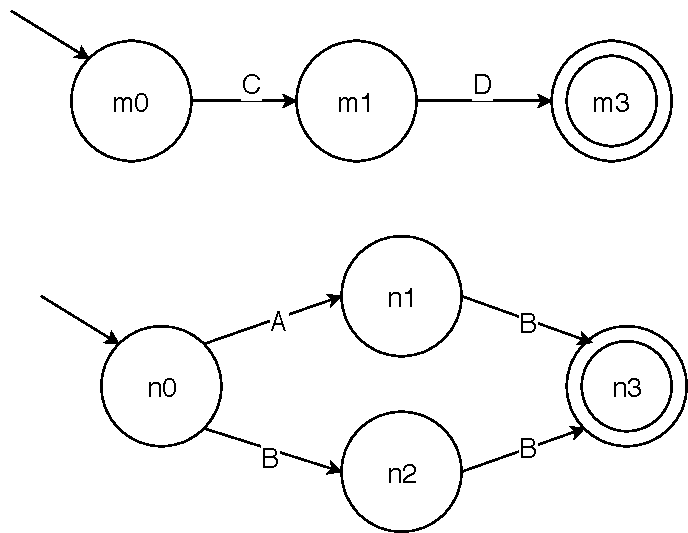
\includegraphics[width=0.7\textwidth]{obrazky-figures/IsertionPriklad.pdf}
\label{imgExample:insertionTeory}
\caption{Příklad automatů pro Sequential Insertion}
\end{figure}

Nyní nad těmito jazyky budeme chtít provést sekvenční vložení $N$ do $M$, tedy \\
$SequentialInsertion(M,N)$. Zde je si potřeba uvědomit, že můžeme provést kartézský součin k tomu abychom sledovali ve kterém jsme právě automatu. Pro jednodušší pochopení si
představme, že automat $M$ je osa $X$ a automat $N$ je osa $Y$. Sekvenční vložení nám pak říká, že musíme řetězec přijímaný automatem $N$ můžeme vložit kamkoliv do řetězce přijímaného automatem $M$. Tedy se můžeme pohybovat přechody po ose $X$
libovolně, ale ve chvíli, kdy se přesuneme po ose $Y$, musíme po této ose dojít až na konec řetězce přijímaného automatem $N$. (viz. \ref{imgExample:insertionTeoryRes})

\begin{figure}[H]
\centering
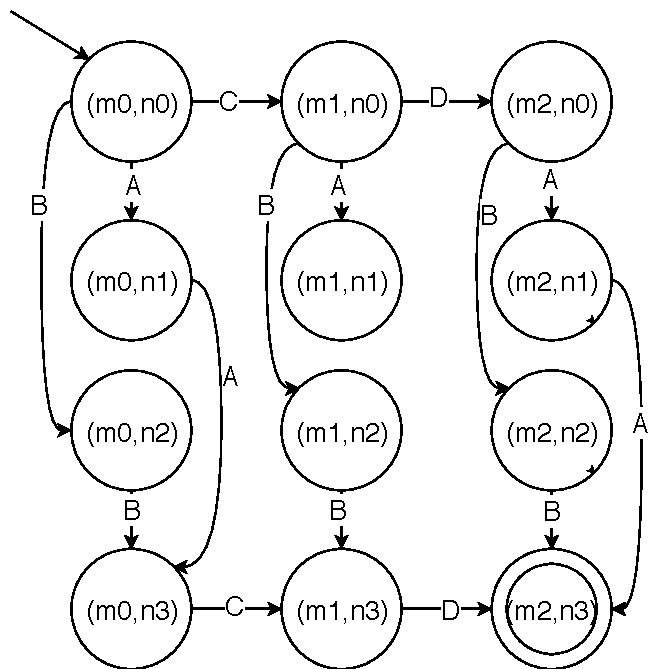
\includegraphics[width=0.7\textwidth]{obrazky-figures/IsertionPrikladResult.pdf}
\label{imgExample:insertionTeoryRes}
\caption{Výsledek po použití operace Sequential Insertion}
\end{figure}



Tento příklad si můžeme zobecnit následujícím způsobem, mějme dva automaty :

$M=\{Q_{M}, \Sigma_{M}, R_{M},s_{M}, F_{M}\}$ a $N=\{Q_{N}, \Sigma_{N}, R_{N},s_{N}, F_{N}\} $

Sekvenční vložení N do M provedeme následovně:
\begin{equation}
\label{eqA:Insertion}
\begin{split}
    Insertion(M,N) = \{ &\\
           &Q = Q_{M} \times Q_{N},\\
    &  \Sigma = \Sigma_{M} \cup \Sigma_{N} \\
    & \delta = \{ (q_{M},q_{N})\alpha \longrightarrow \left\{\begin{matrix}
 (q_{M}\alpha, q_{N})& if & q_{N}=s \vee q_N \in F_{N}\\ 
 (q_{M}, q_{N}\alpha)& else & 
\end{matrix}\right.;\\
    &\tab q_{M} \in Q_{M} \land q_{N} \in Q_{N} \land \alpha \in \Sigma\\
    &\tab\}, \\
    & s = (s_{M}, s_{N}), \\
    & F = F_{M} \times F_{N} \\
    \}&
\end{split}
\end{equation}


\subsection{Implementace}
Pravidla se vytváří dle výše uvedeného automatu, obdobně jako tomu bylo v ukázce \ref{example:shuffle}
(\textit{src/operations/sequentialInsertionFA.js})
% \begin{figure}[h]
% \centering
% \includegraphics[width=0.7\textwidth]{obrazky-figures/intersectionExample.png}
% \label{imgExample:intersection}
% \caption[]
%     {\tabular[t]{@{}l@{}}Ukázka implementace operace Intersection \\ $src/operations/intersectionFA.js$\endtabular}
% \end{figure}

\section{Paralelní vkládání (Paralel Insertion)}
\subsection{Provedení nad automatem}
Provedení paralelního vkládání je velice podobné vkládání sekvenčnímu, nejednodušší bude opět si uvést příklad. Mějme tedy opět dva jazyky $K(M)=\{CD\}$ a $L(N)=\{AA, BB\}$ a automaty kterými jsou definovány, viz výše uvedený příklad pro sekvenční vkládání(\ref{imgExample:insertionTeory});

Rozdíl je zde v tom, že při paralelním vkládání, musíme vždy po zpracování znaku z řetězce jazyka $K(M)$, zpracovat celý řetězec z jazyka $L(N)$. Abychom použili analogii na na osy $X$ a $Y$, tak vždy když se chceme posunout po ose $X$, musíme se posunout po ose $Y$ až do konečného stavu. (viz \ref{imgExample:paralelinsertionResult})
\begin{figure}[H]
\centering
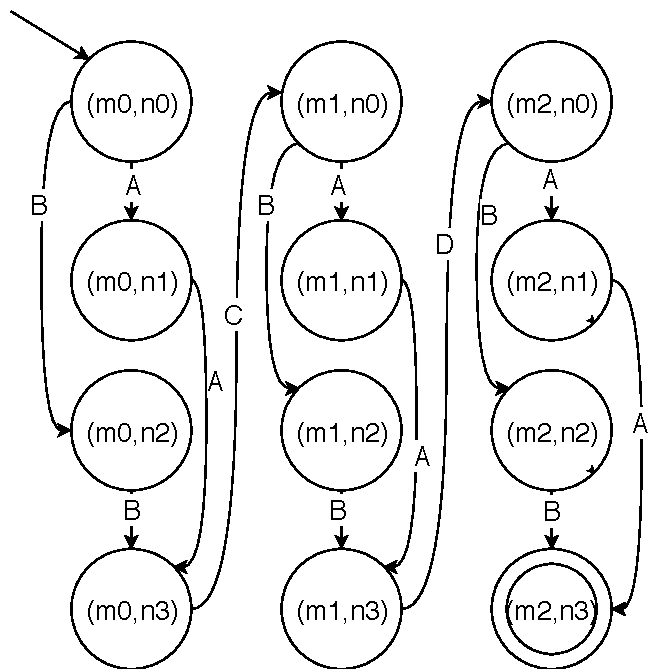
\includegraphics[width=0.7\textwidth]{obrazky-figures/paralelInserionResult.pdf}
\label{imgExample:paralelinsertionResult}
\caption{Automat generovaný operací ParalelInsertion(N,L)}
\end{figure}

Tento příklad si můžeme zobecnit následujícím způsobem, mějme dva automaty :
$M=\{Q_{M}, \Sigma_{M}, \delta_{M},s_{M}, F_{M}\}$ a $N=\{Q_{N}, \Sigma_{N}, \delta_{N},s_{N}, F_{N}\} $

Paralelní vkládání poté můžeme zobecnit následovně:
\begin{equation}
\label{eqA:ParalelInsertion}
\begin{split}
    ParalelInsertion(M,N) = \{ &\\
           &Q = Q_{M} \times Q_{N},\\
    &  \Sigma = \Sigma_{M} \cup \Sigma_{N} \\
    & \delta = \{ (q_{M},q_{N})\alpha \longrightarrow \left\{\begin{matrix}
 (q_{M}\alpha, s_{N})& if & q_N \in F_{N}\\ 
 (q_{M}, q_{N}\alpha)& else & 
\end{matrix}\right.;\\
    &\tab q_{M} \in Q_{M} \land q_{N} \in Q_{N} \land \alpha \in \Sigma\\
    &\tab\}, \\
    & s = (s_{M}, s_{N}), \\
    & F = F_{M} \times F_{N} \\
    \}&
\end{split}
\end{equation}



\subsection{Implementace}
Pravidla se vytváří dle výše uvedeného automatu, obdobně jako tomu bylo v ukázce \ref{example:shuffle}
(\textit{src/operations/parallelInsertionFA.js})
% \begin{figure}[h]
% \centering
% \includegraphics[width=0.7\textwidth]{obrazky-figures/intersectionExample.png}
% \label{imgExample:intersection}
% \caption[]
%     {\tabular[t]{@{}l@{}}Ukázka implementace operace Intersection \\ $src/operations/intersectionFA.js$\endtabular}
% \end{figure}

\section{Protkání (Interlacement)}
V této operaci postupujeme tak, že vytváříme automat přesně tak jak je automat vytvořen v důkazu.
\subsection{Implementace}
Pravidla se vytváří dle výše uvedeného automatu, obdobně jako tomu bylo v ukázce \ref{example:shuffle}
(\textit{src/operations/interlacementFA.js})
\section{Sekvenční mazání (Sequential Deletion)}
[TODO, implementovat, poté popsat]
\section{Zakázání abecedy (Full Alphabet deletion)}
[TODO, implementovat, poté popsat]
[Ale v podstatě se jedná o homomorfismus alpha -> epsilon]
\section{(Pop)}
[TODO, implementovat, poté popsat]
[Ale v podstatě se jedná o homomorfismus alpha -> epsilon]
  
\chapter{Závěr}
TODO
  
  
  % Kompilace po částech (viz výše, nutno odkomentovat)
  % Compilation piecewise (see above, it is necessary to uncomment it)
  %\subfile{projekt-01-uvod-introduction}
  % ...
  %\subfile{chapters/projekt-05-conclusion}


  % Pouzita literatura / Bibliography
  % ----------------------------------------------
\ifslovak
  \makeatletter
  \def\@openbib@code{\addcontentsline{toc}{chapter}{Literatúra}}
  \makeatother
  \bibliographystyle{bib-styles/czechiso}
\else
  \ifczech
    \makeatletter
    \def\@openbib@code{\addcontentsline{toc}{chapter}{Literatura}}
    \makeatother
    \bibliographystyle{bib-styles/czechiso}
  \else 
    \makeatletter
    \def\@openbib@code{\addcontentsline{toc}{chapter}{Bibliography}}
    \makeatother
    \bibliographystyle{bib-styles/englishiso}
  %  \bibliographystyle{alpha}
  \fi
\fi
  \begin{flushleft}
  \bibliography{projekt-20-literatura-bibliography}
  \end{flushleft}

  % vynechani stranky v oboustrannem rezimu
  % Skip the page in the two-sided mode
  \iftwoside
    \cleardoublepage
  \fi

  % Prilohy / Appendices
  % ---------------------------------------------
  \appendix
\ifczech
  \renewcommand{\appendixpagename}{Přílohy}
  \renewcommand{\appendixtocname}{Přílohy}
  \renewcommand{\appendixname}{Příloha}
\fi
\ifslovak
  \renewcommand{\appendixpagename}{Prílohy}
  \renewcommand{\appendixtocname}{Prílohy}
  \renewcommand{\appendixname}{Príloha}
\fi
%  \appendixpage

% vynechani stranky v oboustrannem rezimu
% Skip the page in the two-sided mode
%\iftwoside
%  \cleardoublepage
%\fi
  
\ifslovak
%  \section*{Zoznam príloh}
%  \addcontentsline{toc}{section}{Zoznam príloh}
\else
  \ifczech
%    \section*{Seznam příloh}
%    \addcontentsline{toc}{section}{Seznam příloh}
  \else
%    \section*{List of Appendices}
%    \addcontentsline{toc}{section}{List of Appendices}
  \fi
\fi
  \startcontents[chapters]
  \setlength{\parskip}{0pt}
  % seznam příloh / list of appendices
  % \printcontents[chapters]{l}{0}{\setcounter{tocdepth}{2}}
  
  \ifODSAZ
    \setlength{\parskip}{0.5\bigskipamount}
  \else
    \setlength{\parskip}{0pt}
  \fi
  
  % vynechani stranky v oboustrannem rezimu
  \iftwoside
    \cleardoublepage
  \fi
  
  % Přílohy / Appendices
%  \input{projekt-30-prilohy-appendices}
  
  % Kompilace po částech (viz výše, nutno odkomentovat)
  % Compilation piecewise (see above, it is necessary to uncomment it)
  %\subfile{projekt-30-prilohy-appendices}
  
\end{document}
